\documentclass{article}

% Idioma y codificación
\usepackage[spanish, es-tabla]{babel}       %es-tabla para que se titule "Tabla"
\usepackage[utf8]{inputenc}

% Márgenes
\usepackage[a4paper,top=3cm,bottom=2.5cm,left=3cm,right=3cm]{geometry}

% Comentarios de bloque
\usepackage{verbatim}

% Paquetes de links
\usepackage[hidelinks]{hyperref}    % Permite enlaces
\usepackage{url}                    % redirecciona a la web

% Más opciones para enumeraciones
\usepackage{enumitem}

% Personalizar la portada
\usepackage{titling}


% Paquetes de tablas
\usepackage{multirow}


%------------------------------------------------------------------------

%Paquetes de figuras
\usepackage{caption}
\usepackage{subcaption} % Figuras al lado de otras
\usepackage{float}      % Poner figuras en el sitio indicado H.


% Paquetes de imágenes
\usepackage{graphicx}       % Paquete para añadir imágenes
\usepackage{transparent}    % Para manejar la opacidad de las figuras

% Paquete para usar colores
\usepackage[dvipsnames]{xcolor}
\usepackage{pagecolor}      % Para cambiar el color de la página

% Habilita tamaños de fuente mayores
\usepackage{fix-cm}


%------------------------------------------------------------------------

% Paquetes de matemáticas
\usepackage{mathtools, amsfonts, amssymb, mathrsfs}
\usepackage[makeroom]{cancel}     % Simplificar tachando
\usepackage{polynom}    % Divisiones y Ruffini
\usepackage{units} % Para poner fracciones diagonales con \nicefrac

\usepackage{pgfplots}   %Representar funciones
\pgfplotsset{compat=1.18}  % Versión 1.18

\usepackage{tikz-cd}    % Para usar diagramas de composiciones
\usetikzlibrary{calc}   % Para usar cálculo de coordenadas en tikz

%Definición de teoremas, etc.
\usepackage{amsthm}
%\swapnumbers   % Intercambia la posición del texto y de la numeración

\theoremstyle{plain}

\makeatletter
\@ifclassloaded{article}{
  \newtheorem{teo}{Teorema}[section]
}{
  \newtheorem{teo}{Teorema}[chapter]  % Se resetea en cada chapter
}
\makeatother

\newtheorem{coro}{Corolario}[teo]           % Se resetea en cada teorema
\newtheorem{prop}[teo]{Proposición}         % Usa el mismo contador que teorema
\newtheorem{lema}[teo]{Lema}                % Usa el mismo contador que teorema

\theoremstyle{remark}
\newtheorem*{observacion}{Observación}

\theoremstyle{definition}

\makeatletter
\@ifclassloaded{article}{
  \newtheorem{definicion}{Definición} [section]     % Se resetea en cada chapter
}{
  \newtheorem{definicion}{Definición} [chapter]     % Se resetea en cada chapter
}
\makeatother

\newtheorem*{notacion}{Notación}
\newtheorem*{ejemplo}{Ejemplo}
\newtheorem*{ejercicio*}{Ejercicio}             % No numerado
\newtheorem{ejercicio}{Ejercicio} [section]     % Se resetea en cada section


% Modificar el formato de la numeración del teorema "ejercicio"
\renewcommand{\theejercicio}{%
  \ifnum\value{section}=0 % Si no se ha iniciado ninguna sección
    \arabic{ejercicio}% Solo mostrar el número de ejercicio
  \else
    \thesection.\arabic{ejercicio}% Mostrar número de sección y número de ejercicio
  \fi
}


% \renewcommand\qedsymbol{$\blacksquare$}         % Cambiar símbolo QED
%------------------------------------------------------------------------

% Paquetes para encabezados
\usepackage{fancyhdr}
\pagestyle{fancy}
\fancyhf{}

\newcommand{\helv}{ % Modificación tamaño de letra
\fontfamily{}\fontsize{12}{12}\selectfont}
\setlength{\headheight}{15pt} % Amplía el tamaño del índice


%\usepackage{lastpage}   % Referenciar última pag   \pageref{LastPage}
\fancyfoot[C]{\thepage}

%------------------------------------------------------------------------

% Conseguir que no ponga "Capítulo 1". Sino solo "1."
\makeatletter
\@ifclassloaded{book}{
  \renewcommand{\chaptermark}[1]{\markboth{\thechapter.\ #1}{}} % En el encabezado
    
  \renewcommand{\@makechapterhead}[1]{%
  \vspace*{50\p@}%
  {\parindent \z@ \raggedright \normalfont
    \ifnum \c@secnumdepth >\m@ne
      \huge\bfseries \thechapter.\hspace{1em}\ignorespaces
    \fi
    \interlinepenalty\@M
    \Huge \bfseries #1\par\nobreak
    \vskip 40\p@
  }}
}
\makeatother

%------------------------------------------------------------------------
% Paquetes de cógido
\usepackage{minted}
\renewcommand\listingscaption{Código fuente}

\usepackage{fancyvrb}
% Personaliza el tamaño de los números de línea
\renewcommand{\theFancyVerbLine}{\small\arabic{FancyVerbLine}}

% Estilo para C++
\newminted{cpp}{
    frame=lines,
    framesep=2mm,
    baselinestretch=1.2,
    linenos,
    escapeinside=||
}



\usepackage{listings} % Para incluir código desde un archivo

\renewcommand\lstlistingname{Código Fuente}
\renewcommand\lstlistlistingname{Índice de Códigos Fuente}

% Definir colores
\definecolor{vscodepurple}{rgb}{0.5,0,0.5}
\definecolor{vscodeblue}{rgb}{0,0,0.8}
\definecolor{vscodegreen}{rgb}{0,0.5,0}
\definecolor{vscodegray}{rgb}{0.5,0.5,0.5}
\definecolor{vscodebackground}{rgb}{0.97,0.97,0.97}
\definecolor{vscodelightgray}{rgb}{0.9,0.9,0.9}

% Configuración para el estilo de C similar a VSCode
\lstdefinestyle{vscode_C}{
  backgroundcolor=\color{vscodebackground},
  commentstyle=\color{vscodegreen},
  keywordstyle=\color{vscodeblue},
  numberstyle=\tiny\color{vscodegray},
  stringstyle=\color{vscodepurple},
  basicstyle=\scriptsize\ttfamily,
  breakatwhitespace=false,
  breaklines=true,
  captionpos=b,
  keepspaces=true,
  numbers=left,
  numbersep=5pt,
  showspaces=false,
  showstringspaces=false,
  showtabs=false,
  tabsize=2,
  frame=tb,
  framerule=0pt,
  aboveskip=10pt,
  belowskip=10pt,
  xleftmargin=10pt,
  xrightmargin=10pt,
  framexleftmargin=10pt,
  framexrightmargin=10pt,
  framesep=0pt,
  rulecolor=\color{vscodelightgray},
  backgroundcolor=\color{vscodebackground},
}

%------------------------------------------------------------------------

% Comandos definidos
\newcommand{\bb}[1]{\mathbb{#1}}
\newcommand{\cc}[1]{\mathcal{#1}}

% I prefer the slanted \leq
\let\oldleq\leq % save them in case they're every wanted
\let\oldgeq\geq
\renewcommand{\leq}{\leqslant}
\renewcommand{\geq}{\geqslant}

% Si y solo si
\newcommand{\sii}{\iff}

% Letras griegas
\newcommand{\eps}{\epsilon}
\newcommand{\veps}{\varepsilon}
\newcommand{\lm}{\lambda}

\newcommand{\ol}{\overline}
\newcommand{\ul}{\underline}
\newcommand{\wt}{\widetilde}
\newcommand{\wh}{\widehat}

\let\oldvec\vec
\renewcommand{\vec}{\overrightarrow}

% Derivadas parciales
\newcommand{\del}[2]{\frac{\partial #1}{\partial #2}}
\newcommand{\Del}[3]{\frac{\partial^{#1} #2}{\partial^{#1} #3}}
\newcommand{\deld}[2]{\dfrac{\partial #1}{\partial #2}}
\newcommand{\Deld}[3]{\dfrac{\partial^{#1} #2}{\partial^{#1} #3}}


\newcommand{\AstIg}{\stackrel{(\ast)}{=}}
\newcommand{\Hop}{\stackrel{L'H\hat{o}pital}{=}}

\newcommand{\red}[1]{{\color{red}#1}} % Para integrales, destacar los cambios.

% Método de integración
\newcommand{\MetInt}[2]{
    \left[\begin{array}{c}
        #1 \\ #2
    \end{array}\right]
}

% Declarar aplicaciones
% 1. Nombre aplicación
% 2. Dominio
% 3. Codominio
% 4. Variable
% 5. Imagen de la variable
\newcommand{\Func}[5]{
    \begin{equation*}
        \begin{array}{rrll}
            #1:& #2 & \longrightarrow & #3\\
               & #4 & \longmapsto & #5
        \end{array}
    \end{equation*}
}

%------------------------------------------------------------------------

% Define a custom command for email addresses
\newcommand{\email}[1]{\href{mailto:#1}{{{\color{blue}#1}}}}

\usepackage{schemata}
\usepackage{ragged2e}


\definecolor{codegreen}{rgb}{0,0.6,0}
\definecolor{codegray}{rgb}{0.5,0.5,0.5}
\definecolor{codepurple}{rgb}{0.58,0,0.82}
\definecolor{backcolour}{rgb}{0.95,0.95,0.92}

\definecolor{backcolor}{RGB}{30,30,30}
\definecolor{codeblue}{RGB}{153,255,255}
\definecolor{codepink}{RGB}{200,80,180}
\definecolor{normalblue}{RGB}{12,144,244}

\lstdefinestyle{vscodestyle0}{
    backgroundcolor=\color{backcolor},   
    commentstyle=\color{codegreen},
    keywordstyle=\color{codepink},
    numberstyle=\tiny\color{codegray},
    identifierstyle=\color{codeblue},
    rulecolor=\color{black},
    stringstyle=\color{codepurple},
    basicstyle=\ttfamily\footnotesize,
    breakatwhitespace=false,         
    breaklines=true,                 
    captionpos=b,                    
    keepspaces=true,                 
    numbers=left,                    
    numbersep=5pt,                  
    showspaces=false,                
    showstringspaces=false,
    showtabs=false,                  
    tabsize=2,
    literate=%
  {\ +\ }{{{\color{Red}\ +\ }}}1
  {\ -\ }{{{\color{Red}\ -\ }}}1
  {\ \cdot\ }{{{\color{Red}\ \cdot\ }}}1
  {\ /\ }{{{\color{Red}\ /\ }}}1
  {\ =\ }{{{\color{Red}\ =\ }}}1
}

\lstdefinestyle{vscodestyle}{
    backgroundcolor=\color{backcolor},    % Fondo oscuro
    basicstyle=\color{white}\ttfamily\footnotesize, % Texto en blanco
    commentstyle=\color{green!50!black}, % Estilo de comentarios
    keywordstyle=\color{codepink},       % Estilo de palabras clave
    keywordstyle={[2]\color{blue}}, % Estilo para tipos de datos (int, char, double, etc.)
    identifierstyle=\color{codeblue},
    numberstyle=\tiny\color{gray},   % Estilo de números de línea
    stringstyle=\color{orange},      % Estilo de cadenas de texto
    rulecolor=\color{black},
    breakatwhitespace=false,         % Romper líneas solo en espacios en blanco
    breaklines=true,                 % Romper líneas automáticamente
    captionpos=b,                    % Posición de la leyenda (abajo)
    keepspaces=true,                 % Conservar espacios en blanco
    numbers=left,                    % Mostrar números de línea a la izquierda
    numbersep=5pt,                   % Separación de números de línea del código
    showspaces=false,                % Mostrar espacios con guiones bajos
    showstringspaces=false,          % No subrayar espacios en cadenas de texto
    showtabs=false,                  % No mostrar tabulaciones
    tabsize=4                        % Tamaño de la tabulación
}

\lstset{
    language=C,
    morekeywords={int,char,ld,double}
}


\lstdefinestyle{mystyle}{
    backgroundcolor=\color{backcolour},   
    commentstyle=\color{codegreen},
    keywordstyle=\color{magenta},
    numberstyle=\tiny\color{codegray},
    stringstyle=\color{codepurple},
    %identifierstyle=\color{blue},
    basicstyle=\ttfamily\footnotesize,
    breakatwhitespace=false,         
    breaklines=true,                 
    captionpos=b,                    
    keepspaces=true,                 
    numbers=left,                    
    numbersep=5pt,                  
    showspaces=false,                
    showstringspaces=false,
    showtabs=false,                  
    tabsize=2
}
%\usemintedstyle[C++]{default}
\lstset{style=mystyle}

\newcommand{\myparagraph}[1]{\paragraph{#1}\mbox{}\\}
\newcommand\N{\ensuremath{\mathbb N}\space} 

%REPARTO DE TAREAS%
%    P1:
%        PROSA: DANI
%        EFICIENCIA ESPEC: ALQUI
%        EFICIENCIA DV: LAURA
%        \text{UMBRAL}ES: ALQUI (TODOS) (@LAURA)
%    P2:
%        PROSA: ELIAS
%        EFICIENCIA ESPECIFICO: ELIAS
%        EFICIENCIA DYV: OLGA
%        \text{UMBRAL}ES: LAURA (ELIAS)
%    P3:
%        PROSA: LAURA
%        EFICIENCIA ESPEC: DANI
%        EFICIENCIA DV: OLGA
%        \text{UMBRAL}ES: DANI (OLGA)


\hypersetup{
    colorlinks=false, % Establece 'true' si quieres que el texto del enlace sea de color en lugar de tener un cuadro
    pdfborder={0 0 0}, % Establece el borde del enlace a 0 para eliminarlo
}


\graphicspath{ {images/} }



\begin{document}

    % 1. Foto de fondo
    % 2. Título
    % 3. Encabezado Izquierdo
    % 4. Color de fondo
    % 5. Coord x del titulo
    % 6. Coord y del titulo
    % 7. Fecha
    % 8. Autor

    
    % 1. Foto de fondo
% 2. Título
% 3. Encabezado Izquierdo
% 4. Color de fondo
% 5. Coord x del titulo
% 6. Coord y del titulo
% 7. Fecha

\newcommand{\portada}[7]{

    \portadaBase{#1}{#2}{#3}{#4}{#5}{#6}{#7}
    \portadaBook{#1}{#2}{#3}{#4}{#5}{#6}{#7}
}

\newcommand{\portadaExamen}[7]{

    \portadaBase{#1}{#2}{#3}{#4}{#5}{#6}{#7}
    \portadaArticle{#1}{#2}{#3}{#4}{#5}{#6}{#7}
}




\newcommand{\portadaBase}[7]{

    % Tiene la portada principal y la licencia Creative Commons
    
    % 1. Foto de fondo
    % 2. Título
    % 3. Encabezado Izquierdo
    % 4. Color de fondo
    % 5. Coord x del titulo
    % 6. Coord y del titulo
    % 7. Fecha
    
    
    \thispagestyle{empty}               % Sin encabezado ni pie de página
    \newgeometry{margin=0cm}        % Márgenes nulos para la primera página
    
    
    % Encabezado
    \fancyhead[L]{\helv #3}
    \fancyhead[R]{\helv \nouppercase{\leftmark}}
    
    
    \pagecolor{#4}        % Color de fondo para la portada
    
    \begin{figure}[p]
        \centering
        \transparent{0.3}           % Opacidad del 30% para la imagen
        
        \includegraphics[width=\paperwidth, keepaspectratio]{assets/#1}
    
        \begin{tikzpicture}[remember picture, overlay]
            \node[anchor=north west, text=white, opacity=1, font=\fontsize{60}{90}\selectfont\bfseries\sffamily, align=left] at (#5, #6) {#2};
            
            \node[anchor=south east, text=white, opacity=1, font=\fontsize{12}{18}\selectfont\sffamily, align=right] at (9.7, 3) {\textbf{\href{https://losdeldgiim.github.io/}{Los Del DGIIM}}};
            
            \node[anchor=south east, text=white, opacity=1, font=\fontsize{12}{15}\selectfont\sffamily, align=right] at (9.7, 1.8) {Doble Grado en Ingeniería Informática y Matemáticas\\Universidad de Granada};
        \end{tikzpicture}
    \end{figure}
    
    
    \restoregeometry        % Restaurar márgenes normales para las páginas subsiguientes
    \pagecolor{white}       % Restaurar el color de página
    
    
    \newpage
    \thispagestyle{empty}               % Sin encabezado ni pie de página
    \begin{tikzpicture}[remember picture, overlay]
        \node[anchor=south west, inner sep=3cm] at (current page.south west) {
            \begin{minipage}{0.5\paperwidth}
                \href{https://creativecommons.org/licenses/by-nc-nd/4.0/}{
                    
\includegraphics[height=2cm]{assets/Licencia.png}
                }\vspace{1cm}\\
                Esta obra está bajo una
                \href{https://creativecommons.org/licenses/by-nc-nd/4.0/}{
                    Licencia Creative Commons Atribución-NoComercial-SinDerivadas 4.0 Internacional (CC BY-NC-ND 4.0).
                }\\
    
                Eres libre de compartir y redistribuir el contenido de esta obra en cualquier medio o formato, siempre y cuando des el crédito adecuado a los autores originales y no persigas fines comerciales. 
            \end{minipage}
        };
    \end{tikzpicture}
    
    
    
    % 1. Foto de fondo
    % 2. Título
    % 3. Encabezado Izquierdo
    % 4. Color de fondo
    % 5. Coord x del titulo
    % 6. Coord y del titulo
    % 7. Fecha


}


\newcommand{\portadaBook}[7]{

    % 1. Foto de fondo
    % 2. Título
    % 3. Encabezado Izquierdo
    % 4. Color de fondo
    % 5. Coord x del titulo
    % 6. Coord y del titulo
    % 7. Fecha

    % Personaliza el formato del título
    \pretitle{\begin{center}\bfseries\fontsize{42}{56}\selectfont}
    \posttitle{\par\end{center}\vspace{2em}}
    
    % Personaliza el formato del autor
    \preauthor{\begin{center}\Large}
    \postauthor{\par\end{center}\vfill}
    
    % Personaliza el formato de la fecha
    \predate{\begin{center}\huge}
    \postdate{\par\end{center}\vspace{2em}}
    
    \title{#2}
    \author{\href{https://losdeldgiim.github.io/}{Los Del DGIIM}}
    \date{Granada, #7}
    \maketitle
    
    \tableofcontents
}




\newcommand{\portadaArticle}[7]{

    % 1. Foto de fondo
    % 2. Título
    % 3. Encabezado Izquierdo
    % 4. Color de fondo
    % 5. Coord x del titulo
    % 6. Coord y del titulo
    % 7. Fecha

    % Personaliza el formato del título
    \pretitle{\begin{center}\bfseries\fontsize{42}{56}\selectfont}
    \posttitle{\par\end{center}\vspace{2em}}
    
    % Personaliza el formato del autor
    \preauthor{\begin{center}\Large}
    \postauthor{\par\end{center}\vspace{3em}}
    
    % Personaliza el formato de la fecha
    \predate{\begin{center}\huge}
    \postdate{\par\end{center}\vspace{5em}}
    
    \title{#2}
    \author{\href{https://losdeldgiim.github.io/}{Los Del DGIIM}}
    \date{Granada, #7}
    \thispagestyle{empty}               % Sin encabezado ni pie de página
    \maketitle
    \vfill
}
    \portada{etsiitA4.jpg}{Algorítmica\\Práctica 2}{Algorítmica. Práctica 2. DyV.}{MidnightBlue}{-8}{28}{2023-2024}{Laura Mandow Fuentes\\Chengcheng Liu\\Daniel Hidalgo Chica\\Roberto González Lugo\\Elías Monge Sánchez}

    \newpage

    
\section{Participación}
    \begin{itemize}
        \item Laura Mandow Fuentes. \email{e.lauramandow@go.ugr.es}  $100\%$
        \item Roberto González Lugo. \email{e.roberlks222@go.ugr.es}  $100\%$
        \item Daniel Hidalgo Chica. \email{e.danielhc@go.ugr.es}  $100\%$
        \item Chengcheng Liu. \email{e.cliu04@go.ugr.es} $100\%$
        \item Elías Monge Sánchez. \email{e.eliasmonge234@go.ugr.es}  $100\%$
    \end{itemize}
    \subsection{Participación específica}
    Aunque hayamos trabajado cada uno de forma global los contenidos de la práctica, a la hora de la redacción de la memoria, el trabajo se ha visto dividido en partes de carga de trabajo similar con el fin de aumentar la productividad.
    \\
    En particular, las máquinas utilizadas para ejecutar los algoritmos son:
    \begin{itemize}
        \item P1
        \begin{itemize}
            \item Específico: \begin{itemize}
                \item Máquina: Asus TUF fx505dt
                \item Procesador: AMD Ryzen 7 3750h with Radeon Vega Mobile Gfx 2.3GHz
                \item Tarjeta gráfica: Nvidia Geforce GTX 1650
                \item Sistema Operativo: Arch Linux 64bits

            \end{itemize}
            \item DyV \begin{itemize}
                \item Máquina: Surface Laptop 4
                \item Procesador: Intel Core i7
                \item Tarjeta Gráfica: Intel Corporation TigerLake-LP GT2 [Iris Xe Graphics] (rev 01)
                \item Sistema Operativo: Ubuntu 22.04 64bits
            \end{itemize}
                \item Umbrales\begin{itemize}
                    \item Máquina: Asus TUF fx505dt
                    \item Procesador: AMD Ryzen 7 3750h with Radeon Vega Mobile Gfx 2.3GHz
                    \item Tarjeta gráfica: Nvidia Geforce GTX 1650
                    \item Sistema Operativo: Arch Linux 64bits 
            \end{itemize}
        \end{itemize}
        \item P2
        \begin{itemize}
            \item Específico\begin{itemize}
                \item Máquina: Acer Aspire A315-42
                \item Procesador: Procesador: AMD Ryzen 5 3500U 2.10 GHz
                \item Tarjeta Gráfica: Radeon Vega Mobile Gfx
                \item Sistema Operativo: Ubuntu 22.04 64bits (Oracle VM VirtualBox, 2 cores)
            \end{itemize}
            \item DyV\begin{itemize}
                \item Máquina: Acer Aspire A515-45
                \item Procesador: AMD Ryzen 5 5500U 
                \item Tarjeta Gráfica: AMD Radeon Graphics 7 cores, 1800 MHz


                \item Sistema Operativo: Ubuntu 22.04 64 bits
            \end{itemize}
            \item Umbrales\begin{itemize}
                \item Máquina: Acer Aspire A315-42
                \item Procesador: Procesador: AMD Ryzen 5 3500U 2.10 GHz
                \item Tarjeta Gráfica: Radeon Vega Mobile Gfx
                \item Sistema Operativo: Ubuntu 22.04 64bits (Oracle VM VirtualBox, 2 cores)
            \end{itemize}
        \end{itemize}
        \item P3
        \begin{itemize}
            \item Específico\begin{itemize}
                \item Máquina: HP Laptop 15s-eq1xxx
                \item Procesador:AMD Ryzen 5 4500U with Radeon Graphics
                \item Sistema Operativo: Ubuntu 22.04 64 bits
            \end{itemize}
            \item DyV\begin{itemize}
                \item Máquina: Acer Aspire A515-45
                \item Procesador: AMD Ryzen 5 5500U 
                \item Tarjeta Gráfica: AMD Radeon Graphics 7 cores, 1800 MHz


                \item Sistema Operativo: Ubuntu 22.04 64 bits
            \end{itemize}
                \item Umbrales\begin{itemize}
                \item Máquina: HP Laptop 15s-eq1xxx
                \item Procesador:AMD Ryzen 5 4500U with Radeon Graphics
                \item Sistema Operativo: Ubuntu 22.04 64 bits
            \end{itemize}
        \end{itemize}
    \end{itemize}
        

\section{Objetivos}
Los objetivos de nuestra práctica se centran en comprender y asimilar de manera profunda y sistemática la metodología Divide y Vencerás, aplicada al diseño y desarrollo de algoritmos complejos. Esta metodología, que se basa en descomponer un problema en subproblemas de menor tamaño, más manejables y similares al problema original, se convierte en el eje central de nuestro estudio. Nuestro trabajo, por lo tanto, no solo se orienta hacia el diseño e implementación de diversos algoritmos siguiendo las pautas y requerimientos específicos establecidos en las directrices de la práctica, sino que también busca profundizar en la comprensión teórica y aplicada de esta estrategia de solución de problemas.

Fomentamos así la capacidad de resolver problemas complejos de manera eficiente y efectiva, aplicando los principios de esta técnica de diseño de algoritmos. Además, pretendemos desarrollar una habilidad crítica en la evaluación de las soluciones obtenidas, no solo en términos de su correctitud sino también en términos de eficiencia computacional y optimización de recursos. Esto implica una exploración detallada de cómo la división del problema influye en la complejidad temporal y espacial de los algoritmos diseñados, y cómo se puede lograr un balance entre la simplicidad del diseño y la eficiencia en la ejecución.

Asimismo, otro de nuestros objetivos es fomentar el trabajo colaborativo y el intercambio de ideas dentro del equipo, para potenciar la creatividad en la solución de problemas y la capacidad de adaptación de la metodología a diferentes contextos y tipos de problemas. Buscamos, por ende, no solo la asimilación de conocimientos técnicos sino también el desarrollo de competencias transversales, como el pensamiento crítico, la comunicación efectiva y la gestión del trabajo en equipo.

En conclusión, los objetivos de nuestra práctica abarcan una comprensión exhaustiva de la metodología Divide y Vencerás en el ámbito del diseño de algoritmos, la habilidad para implementar soluciones eficientes y efectivas a problemas complejos, y el desarrollo de habilidades blandas y competencias que complementen nuestra formación técnica. A través de este enfoque integral, buscamos prepararnos no solo para enfrentar desafíos académicos sino también para contribuir de manera significativa en el campo profesional de la ciencia de la computación

\newpage

\section{P1: Subsecuencia de suma máxima}

\subsection{Definición del problema}

    Dado una secuencia de valores reales (positivos o negativos),
    almacenada en un vector, se pide encontrar una subsecuencia de
    elementos consecutivos que cumpla que la suma de los
    elementos de la misma sea la máxima posible. 
    
    Aunque existe el algoritmo de Kadane que permite encontrar de forma
    óptima el valor de dicha subsecuencia en $O(n)$, se pide
    encontrar un algoritmo que siguiendo la estrategia divide
    y vencerás encuentre una solución al problema lo más eficiente
    posible, esto es, con dicho orden de eficiencia.

\subsection{Algoritmo específico} 
\subsubsection{Diseño e implementación}
No sorprende que intentando encontrar solución para el problema de manera
no recursiva y buscando eficiencia, hayamos llegado de manera independiente
a una solución totalmente equivalente al algoritmo de Kadane. En cualquier caso,
merece la pena exponer los razonamientos que nos han derivado a la obtención
de este algoritmo además de una demostración formal de su corrección.

La idea es la siguiente: vamos acumulando en una variable la suma de todos los elementos del vector recorridos hasta el momento, y ponemos a 0 este acumulador cada vez que alcance un valor negativo. Y es que esto nos proporciona una delimitación de la Subsecuencia de Suma Máxima, en tanto que, sea cual sea, no puede contener un valor del vector en el que la acumulación haya sido negativa.

Esto es totalmente intuitivo, como vemos en el caso del primer valor del vector
para el cual el acumulador sea negativo: Si vamos acumulando y la suma de todos
los elementos que llevamos se torna negativa en el elemento $k$-ésimo, una secuencia que comience en el elemento $k+1$-ésimo, nunca aumentaría su suma extendiéndose hacia la izquierda. Se ve claramente en un ejemplo:
\[
[3, 4, 10, -20, 8, 2, ...]
\]
Y apreciamos que cualquier secuencia que comience en el $8$ nunca aumentaría
su suma total al extender hacia la izquierda incluyendo al $-20$ y 
a alguno de los valores a su previos a este.

Proponemos ahora una demostración formal de este hecho, generalizando:

\begin{teo}
Sea $v$ un vector de enteros de $n$ elementos $v = [a_{0}, a_{1}, \ldots, a_{n-1}]$ y una subsecuencia $S = [a_{k}, a_{k+1}, \ldots, a_{k+r-1}]$ de $r$ elementos contenida en $v$. Sea también $A_{s}$ definida como:
\[
A_{s} = 
\begin{cases}
a_{0} &\text{ si } s = 0 \\
A_{s-1} + a_{s} &\text{ si } A_{s-1} + a_{s} \ge 0 \\
0 &\text{ si } A_{s-1} + a_{s} < 0 \\
\end{cases} 
\]
Entonces, si $A_{k-1} = 0$ la subsecuencia $S$ tendrá una suma mayor que cualquier extensión suya hacia la izquierda, es decir:
\[
\sum_{j=k}^{k+r-1} a_{j} \ge \sum_{j=k-m}^{k+r-1} a_{j}, \quad m \in \mathbb{N} : 0 \le m \le k
\] 

\begin{proof}
La demostración es por inducción según el predicado $P(u)$ del tenor:
\begin{center}
    cualquier subsecuencia del vector $v$ que comience en el elemento
    posterior a uno $k$ tal que $A_k = 0$ por $u$-ésima vez, tiene
    mayor suma que cualquier extensión suya hacia la izquierda.
\end{center}
Demostramos el caso $u = 1$, es decir, tenemos una tenemos una subsecuencia $S = [a_{k+1}, a_{k+2}, \ldots, a_{k+r}]$, donde $A_{k} = 0$ por primera vez en el recorrido del vector.
Es decir, tenemos
\begin{align}
a_{0} + a_{1} + a_{2} + \ldots + a_{k} &< 0 \\
a_{0} + a_{1} + a_{2} + \ldots + a_{k-s} & \geq 0 
\end{align}
Para cualquier $s$ natural entre $1$ y $k$. Veamos que esto
implica que $a_{k-s} + a_{k-s+1} + \ldots + a_{k} < 0$ y que por tanto al extender hacia la izquierda la subsecuencia $S$ su suma 
nunca aumenta.
\[
a_{k-s} + a_{k-s+1} + \ldots + a_{k} \le  a_{0} + a_{1} + a_{2} + \ldots + a_{k-s} + a_{k-s+1} + \ldots + a_{k} < 0
\]
Donde la primera desigualdad se da por (2).
\\
\\
Para el caso $u \geq 1$: \\
\noindent
Supongamos como hipótesis de inducción que $P(u-1)$ vale y desarrollamos en dos partes: 
\\
\noindent
En primer lugar, de manera totalmente análoga al caso $u = 1$ demostramos que
la subsecuencia tiene suma mayor que cualquier extensión suya
hacia la izquierda delimitada entre el $k$-ésimo elemento del vector donde $A_{k} = 0$ por $u$-ésima vez y el $j$-ésimo elemento del vector, donde $A_{j} = 0$ por $(u-1)$-ésima vez. Además, por
hipótesis de inducción, tenemos que la subsecuencia también tiene
suma mayor que cualquier extensión suya tomando elementos enteriores al 
$j$-ésimo. Por tanto, se tiene $P(u)$ y por el \textbf{Principio de Inducción Matemática} sabemos que $P(u)$ vale en todos los casos (incluso considerando un vector de infinitos elementos, y por tanto el caso finito queda probado).
\end{proof}

\end{teo}
Por tanto, tenemos que una SSM no puede atravesar un punto en el que la variable acumuladora se anule.
Además, es ahora también evidente que la Subsecuencia de Suma Máxima comenzará en
un valor del vector inmediatamente posterior a uno en el que 
se haya anulado la variable acumuladora, pues de no ser así, podría extenderse hacia la izquierda hasta ese punto aumentando su suma (ya que la suma de esos valores es positiva pues la variable acumuladora no se ha anulado al pasar por ellos). 

Por tanto, para encontrarla entonces no tendremos más que comenzar una posible SSM cada vez que la variable acumuladora valga 0, y actualizar la mejor subsecuencia cuando la suma de la actual sea mayor que la suma de la anterior SSM, obteniendo la verdadera SSM al recorrer el vector al completo.

\subsubsection{Análisis de eficiencia} % Roberto
\myparagraph{Eficiencia Teórica del Algoritmo Específico}

La eficiencia teórica del algoritmo implementado en la función \texttt{lineal}, encargada de calcular la subsecuencia contigua de suma máxima (MCSS) de un array, así como el máximo prefijo, máximo sufijo y la suma total del array, se analiza a continuación. Este análisis se centra en el comportamiento del algoritmo en función del tamaño de entrada $n$, siendo $n$ la longitud del array.


El algoritmo realiza un único recorrido lineal por el array, determinando las métricas mencionadas mediante operaciones de complejidad constante en cada paso. Por lo tanto, la complejidad temporal del algoritmo es directamente proporcional al tamaño del array.

\begin{enumerate}
 
    \item \textbf{Inicialización y Recorrido Lineal:} Al inicio, el algoritmo configura los valores iniciales para MCSS y el máximo prefijo a partir del primer elemento del array. Este proceso de inicialización se realiza en tiempo constante.
    \lstinputlisting[language=C++, firstline=38, lastline=46]{Codigos/P1/especifico.cpp}
    
    
    Durante el recorrido por el array (un bucle \texttt{for} que va desde \texttt{ini} hasta \texttt{fin}), se realizan sumas, comparaciones y actualizaciones de variables que son operaciones de complejidad $O(1)$. Este recorrido permite calcular el MCSS, el máximo prefijo y la suma total del array en tiempo lineal.
    \lstinputlisting[language=C++, firstline=47, lastline=66]{Codigos/P1/especifico.cpp}


    \item \textbf{2ª inicialización}
    Después del recorrido principal, el algoritmo realiza algunas inicializaciones para calcular el sufijo máximo, esto, al igual que en el caso anterior, es constante (O(1))
    \lstinputlisting[language=C++, firstline=68, lastline=78]{Codigos/P1/especifico.cpp} 
    
    \item \textbf{Cálculo de Sufijo Máximo:} Después del recorrido principal y la segunda inicialización, el algoritmo ejecuta otro recorrido desde el final del array hacia el inicio para determinar el sufijo máximo. Al igual que el recorrido anterior, este se realiza en tiempo lineal respecto al tamaño del array.
    \lstinputlisting[language=C++, firstline=79, lastline=88]{Codigos/P1/especifico.cpp}
\end{enumerate}

\textbf{Complejidad Total:} Considerando que ambos recorridos por el array y las operaciones de inicialización y actualización se realizan en tiempo constante, la complejidad total del algoritmo \texttt{"lineal"} \footnote{Evidentemente, es por esto que hemos nombrado a la función de dicha manera} es $O(n)$, donde $n$ es la longitud del array. 

\begin{equation}
    T(n) = O(n)
\end{equation}

Por lo tanto, la eficiencia teórica del algoritmo \texttt{lineal}, responsable de calcular la subsecuencia contigua de suma máxima, máximo prefijo, máximo sufijo y la suma total de un array, se establece como de orden lineal $O(n)$. Esto indica que el tiempo de ejecución del algoritmo crece de manera proporcional al tamaño del problema $n$.

\myparagraph{Eficiencia Empírica del algoritmo específico}
Para realizar el análisis de la eficiencia empírica, basta con realizar múltiples ejecuciones del algoritmo para comprobar de forma práctica (empírica) como se comporta. (Que podemos adelantar, que será de forma lineal tal y como hemos desarrollado formalmente)


\begin{figure}[H]
	\centering
	\begin{subfigure}{0.4\textwidth}
            \centering
            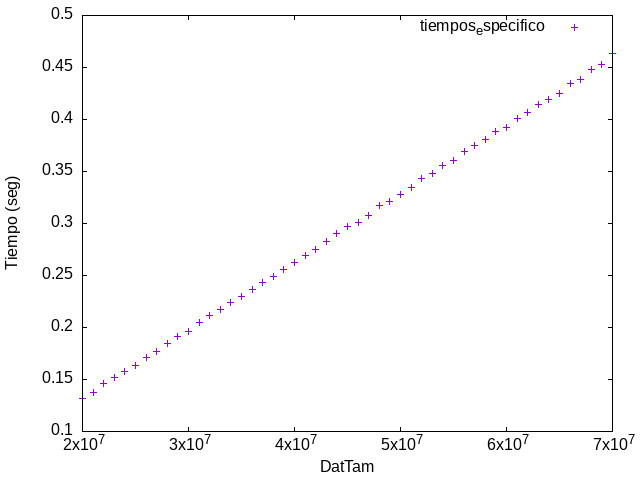
\includegraphics[scale = 0.40]{P1/tiempos_especifico_Puntos.png}
        \end{subfigure}	\hfill
	\begin{subfigure}{0.4\textwidth}
            \centering
            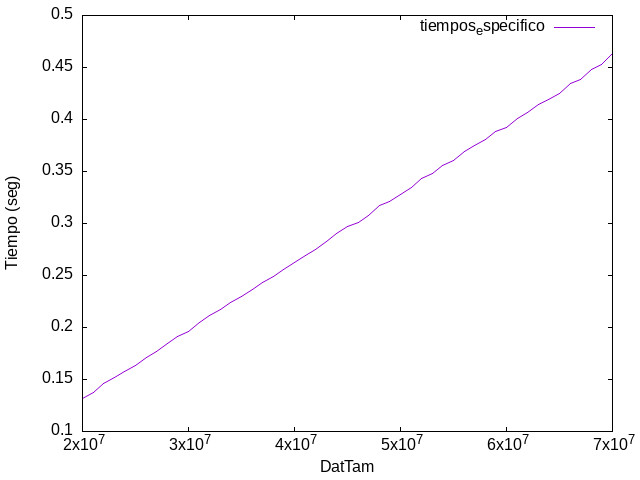
\includegraphics[scale = 0.40]{P1/tiempos_especifico_Lineas.png}
        \end{subfigure}
    \end{figure}

\myparagraph{Eficiencia Híbrida del algoritmo específico}
Es bastante evidente darnos cuenta de que la regresión que debemos aplicar para encontrar el ajuste, obviamente es lineal, confirmando el análisis teórico. Observemoslo:
\begin{figure}[!hbt]
    \centering
    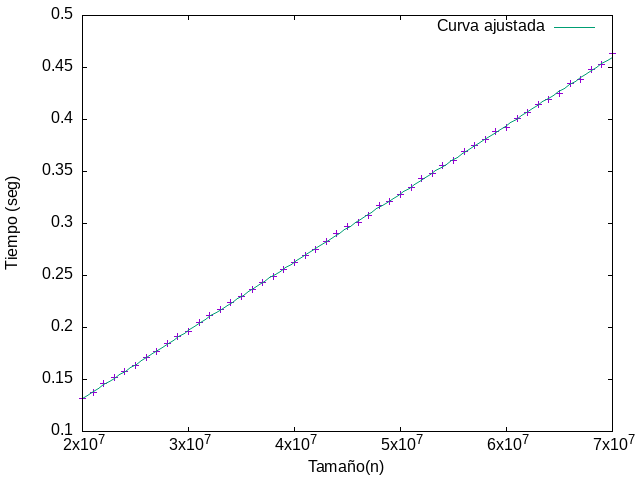
\includegraphics[scale=0.7]{P1/regresion.png}
    \caption{\centering $f(x) = 6.57198\cdot 10^{-9} \cdot x$}
\end{figure}

\subsection{Algoritmo divide y vencerás}


\subsubsection{Diseño e implementación} % Colaborativo
La idea de este algoritmo es más intuitiva si cabe del algoritmo 
lineal: separamos el vector en dos vectores de la mitad del tamaño
original cada uno y calculamos recursivamente en cada uno de ellos:
\begin{itemize}
    \item Su SSM
    \item Su SSM que tenga como primer elemento el primero del array: maxPrefix
    \item Su SSM que tenga como último elemento el último del array: maxSuffix
\end{itemize}

De esta manera, es clara la manera de unir soluciones de ambos
lados del array: la SSM total será la que tenga mayor suma de entre 
\begin{itemize}
    \item La SSM de la izquierda
    \item La SSM de la derecha
    \item La SSM resultante de concatenar maxSuffix de la izquierda con maxPrefix de la derecha
\end{itemize}

Para falcilitar este proceso se usa el tipo de dato sub-secuencia
(con un operador de comparación y de salida) y un tipo de dato
tupla que reune tres secuencias: la SSM, maxPrefix y maxSuffix.
Además, este último tipo también guarda la suma total de los elementos del array que está considerando en ese paso (útil para 
actualizar el valor de maxPrefix y maxSuffix en la fase de
Mezcla de Soluciones).


\lstinputlisting[language=C++, firstline=1, lastline=37]{Codigos/P1/especifico.cpp}

En particular, como no podría ser de otra manera, la forma de
obtener las subsecuencias maxSuffix y maxPrefix en cada caso
iteración es el siguiente:
\begin{itemize}
    \item Para obtener maxPrefix: se obtiene la máxima subsecuencia (en cuanto a suma) entre la \verb+maxPrefix_izquierda+ y la unión de todo el vector izquierdo con \verb+maxPrefix_derecha+.
    \item Para obtener maxSuffix: se obtiene la máxima subsecuencia (en cuanto a suma) entre la \verb+maxSuffix_derecha+ y la unión de todo el vector derecho con \verb+maxSuffix_izquierda+.
\end{itemize}

Usando estas ideas, el código queda de la siguiente manera:
(Ignórense los comentarios)


\lstinputlisting[language=C++, firstline=2, lastline=152]{Codigos/P1/dyv_lineal_array.cpp}


\subsubsection{Análisis de eficiencia} %

\myparagraph{Eficiencia teórica}

Calculemos la eficiencia teórica del algoritmo, es decir, de la función $dyv$.\\

%\inputminted[firstline=92, lastline=97,breaklines,linenos]{C++}{Codigos/P2/dyv_lineal_array.cpp}

\lstinputlisting[language=C++, firstline=92, lastline=97]{Codigos/P1/dyv_lineal_array.cpp}

Observando el código podemos observar un $if/else$ inicial (aunque no haya $else$ explícitamente podemos ver que el resto del código solo se ejecuta cuando no lo hace el $if$ al haber un $return$). Podemos ver que el código del $if$ se ejecuta solo cuando el tamaño del problema ($n = fin - ini$) es menor o igual que la constante $\text{UMBRAL}\in \N$. Estos serían los casos base los cúales se resuelven llamando a la función $lineal$ que consiste en el algoritmo específico previamente detallado cuya eficiencia se vio que era $O(n)$.\\

\lstinputlisting[language=C++, firstline=99, lastline=103]{Codigos/P1/dyv_lineal_array.cpp}

Mientras tanto en el $else$ (caso general) se calcula el punto medio entre $ini$ y $fin$ para luego llamar recursivamente a la función $dyv$. Es decir, se parte el problema por la mitad y se llama recursivamente a la función para resolver cada una de las mitades. \\

\lstinputlisting[language=C++, firstline=105, lastline=152]{Codigos/P1/dyv_lineal_array.cpp}

El resto del código se compone de $if/else$ y operaciones matemáticas las cuales son $O(1)$ y están situadas secuencialemente a las llamadas recursivas previamente mencionadas. 

Por tanto, tenemos que la ecuación de la eficiencia teórica es:
\begin{equation} \label{eq:ef_dyv_p1}
    T(n) = \left\{ \begin{array}{lcc} n & n \leq \text{UMBRAL} &\text{caso base} \\ \\ 2T\left(\nicefrac{n}{2}\right) + 1 & n > \text{UMBRAL} & \text{caso general} \\ \end{array} \right. \hspace{10mm} \forall n \in \N
\end{equation}

Resolvamos la ecuación de recurrencia para obtener la eficiencia del caso general, es decir, $\forall n \in \N$ tal que $n > \text{UMBRAL}$:
\begin{equation}
    T(n) = 2T\left(\nicefrac{n}{2}\right) + 1 \hspace{10mm} \forall n \in \N \hspace{1mm} : \hspace{1mm} n > \text{UMBRAL}
\end{equation}

Desarrollándola en serie $k$ veces, con $k = \log_2\left(\frac{n}{\text{UMBRAL}}\right)$ (aproximando al entero superior) puesto que el problema es de tamaño $n$ y se va subdividiendo por la mitad hasta llegar a un problema de tamaño $\text{UMBRAL}$, tenemos:
\begin{align*}
T(n) &= 2T\left(\nicefrac{n}{2}\right) + 1 = 2(2T\left(\nicefrac{n}{4}\right) + 1) + 1 =
4T\left(\nicefrac{n}{4}\right) + 2 + 1 = 4(2T\left(\nicefrac{n}{8}\right) + 1) + 3 = 
8T\left(\nicefrac{n}{8}\right) + 4 + 3 = \\
&=  8T\left(\nicefrac{n}{8}\right) + 7 = ... = 
2^{k}T\left(\frac{n}{2^{k}}\right) + 2^{k} - 1 = ... = \left\{\text{Sustituimos por } k = \log_2\left(\frac{n}{\text{UMBRAL}}\right) \right\} = \\
&= 2^{\log_2\left(\frac{n}{\text{UMBRAL}}\right)}T\left(\frac{n}{2^{\log_2\left(\frac{n}{\text{UMBRAL}}\right)}}\right) + 2^{\log_2\left(\frac{n}{\text{UMBRAL}}\right)} - 1 = \\
&= \frac{n}{\text{UMBRAL}}T\left(\text{UMBRAL}\right) + \frac{n}{\text{UMBRAL}} - 1 \in O(n)
\end{align*}

Como $T(\text{UMBRAL})$ es constante (por serlo $\text{UMBRAL}$) tenemos que:
\begin{equation}
    \frac{n}{\text{UMBRAL}}T\left(\text{UMBRAL}\right) + \frac{n}{\text{UMBRAL}} - 1 \in O(n)
\end{equation}

Por tanto, recordando la ecuación (\ref{eq:ef_dyv_p1}) tenemos que el orden de eficiencia teórica de este algoritmo es $O(n)$ $\forall n \in \bb{N}$.

\myparagraph{Eficiencia empírica}

Realicemos ahora el estudio de la eficiencia empírica. Para ello, el programa ha sido ejecutado con los valores más grandes posibles, es decir, desde secuencias de tamaño $n = 10000$ hasta $n = 1000000$ cada $39600$.\\
Los tiempos obtenidos para el tamaño de secuencia $n$ se encuentran en la Tabla \ref{tab:time_p1_dyv}. Además se puede observar su representación en las gráficas \ref{fig:p1_dyv_line}
y \ref{fig:p1_dyv_point}.
\begin{table}[]
    \centering
    \begin{tabular}{|c|c|}
            \hline
        Tamaño(n) & Tiempo (seg) \\
        \hline
         10000   &   0.0007313 \\
        49600    &  0.00350708\\
        89200     & 0.00637291\\
        128800     &0.00917196\\
        168400&     0.0121215\\
        208000 &    0.0149036\\
        247600  &   0.0177062\\
        287200   &  0.0207045\\
        326800    & 0.0235259\\
        366400     &0.0264423\\
        406000&     0.0297207\\
        445600 &    0.0324105\\
        485200  &   0.0347352\\
        524800   &  0.0380546\\
        564400    & 0.0411165\\
        604000     &0.0435186\\
        643600&     0.0467262\\
        683200 &    0.0500663\\
        722800  &   0.052286\\
        762400   &  0.0555019\\
        802000    & 0.0571399\\
        841600     &0.0609255\\
        881200&     0.0637417\\
        920800 &    0.0662403\\
        960400  &   0.0695548\\
        1000000  &  0.0719015\\
        \hline
    \end{tabular}
    \caption{\centering Tiempos obtenidos para el algoritmo divide y vencerás del problema 1}
    \label{tab:time_p1_dyv}
\end{table}

\begin{figure}[H]
    \centering
    \begin{subfigure}[b]{0.4\textwidth}
        \centering
        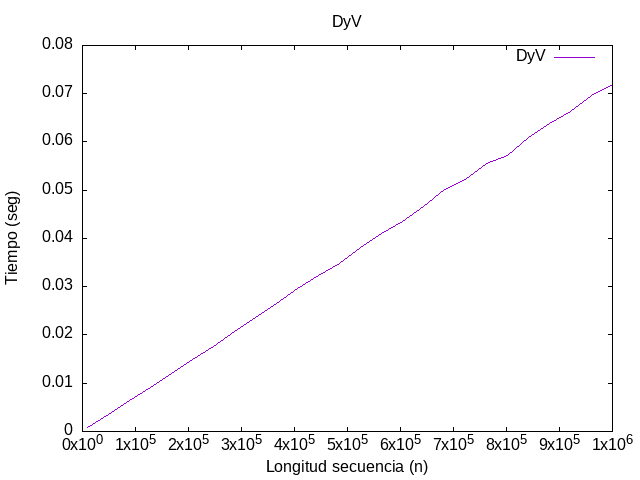
\includegraphics[width=\textwidth]{P1/p1_dyv_lines.png}
        \caption{\centering Gráfica del algoritmo divide y vencerás para el problema 1 (línea)}
        \label{fig:p1_dyv_line}
    \end{subfigure}
    %\hfill
    \begin{subfigure}[b]{0.4\textwidth}
        \centering
        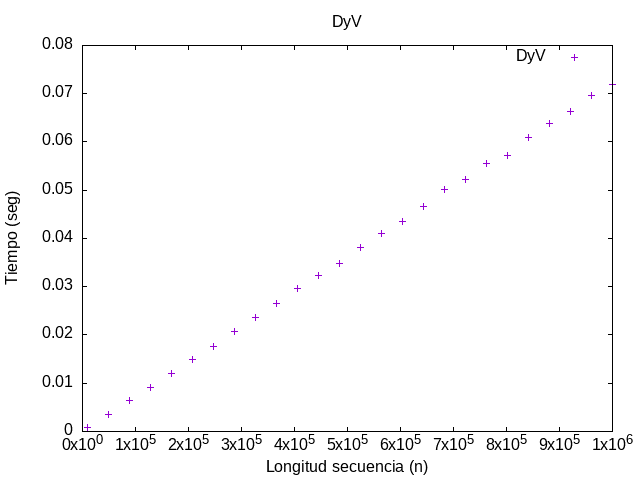
\includegraphics[width=\textwidth]{P1/p1_dyv_points.png}
        \caption{\centering Gráfica del algoritmo divide y vencerás para el problema 1 (puntos)}
        \label{fig:p1_dyv_point}
    \end{subfigure}
\end{figure}

Como se puede observar, se trata de una función claramente lineal, lo que coincide con el resultado demostrado en el análisis teórico.

\myparagraph{Eficiencia híbrida}

Previamente en el análisis teórico se vio que la eficiencia del algoritmo es $O(n)$ y en el análisis empírico constatamos que efectivamente el algoritmo tiene complejidad lineal. \\

Para obtener las constantes ocultas de la ecuación de eficiencia y verificar que en efecto la función que representa la complejidad del algoritmo se trata de una función lineal hemos realizado una regresión lineal por mínimos cuadrados sobre los puntos obtenidos empíricamente con gnuplot, es decir, con una recta de la forma $f(x) = ax + b$.\\

\begin{figure}[H]
    \centering
    \begin{subfigure}[b]{0.4\textwidth}
        \centering
        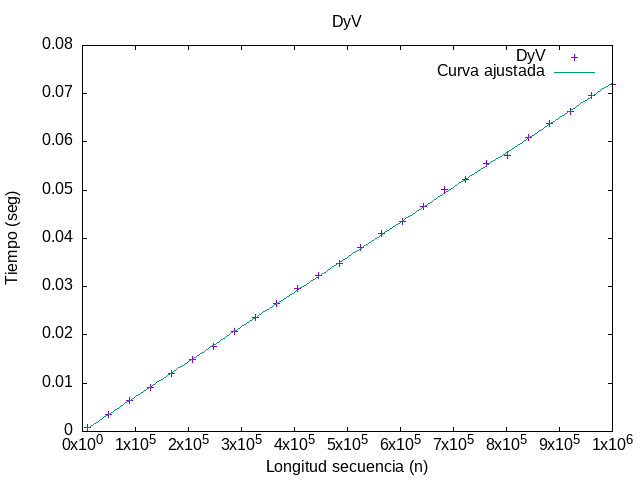
\includegraphics[width=\textwidth]{P1/p1_dyv_ajuste.png}
        \caption{\centering Gráfica ajustada del algoritmo divide y vencerás para el problema 1    }
        \label{fig:p1_dyv_ajuste}
    \end{subfigure}
    \hfill
    \begin{subfigure}[b]{0.5\textwidth}
        \centering
        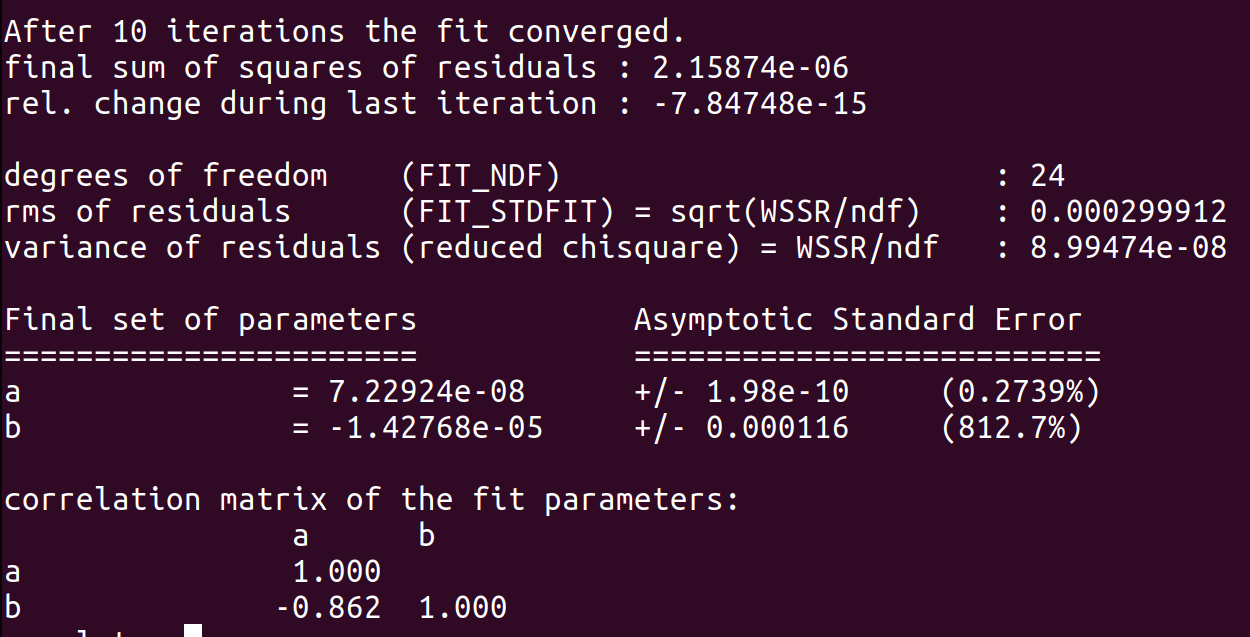
\includegraphics[width=\textwidth]{P1/p1_dyv_fit.png}
        \caption{\centering Regresión lineal del divide y vencerás del problema 1}
        \label{fig:p1_dyv_fit}
    \end{subfigure}
\end{figure}

La función obtenida es:
\begin{equation*}
    f(x) = 7.22924\cdot10^{-8}x - 1.42768 \cdot10^{-5}
\end{equation*}

Como podemos observar en la figura \ref{fig:p1_dyv_fit} la varianza residual es minúscula lo que nos indica que el ajuste realizado es el correcto, tal y como se ve en la gráfica \ref{fig:p1_dyv_ajuste} y por tanto el algoritmo es, en efecto, $O(n)$.

\subsubsection{Cálculo de umbrales} %
    En esta sección calcularemos los umbrales teórico, óptimo y de tanteo,
    para posteriormente compararlos gráficamente. \\

    \myparagraph{Umbral teórico} 
    Para el cálculo del umbral teórico, planteamos la ecuación del algoritmo
    específico tal cual ($h(n)=n$), la aplicamos en el primer nivel de recurrencia y resolvemos la ecuación (no recurrente):

    \begin{equation} \label{eq:ef_dyv_p1}
    T(n) = \left\{ \begin{array}{lcc} n & n \leq \text{UMBRAL}  \\ \\ 
    2T ( \nicefrac{n}{2} ) + 1 &  n > \text{UMBRAL}  \\ \end{array} \right. \hspace{10mm} \forall n \in \N
    \end{equation}

    Entonces nos queda: 
    $$n = 2(\nicefrac{n}{2}) +1 \iff 1=0$$
\[
\]
    Con lo que concluimos que no podemos calcular el umbral teórico
    para este algoritmo. Este resultado se da por tener ambos algoritmos
    el mismo orden de eficiencia, y es una prueba más de que el umbral teórico
    es meramente indicativo. 
    \myparagraph{Umbral óptimo}
    Para el cálculo del umbral óptimo, plantearíamos la función del algoritmo específico obtenida en la eficiciencia híbrida, la aplicaríamos en el primer nivel de recurrencia y resolvemos, pero al igual que con el teórico, esto no tiene sentido ya que ambos algorítmos son de el mismo orden de eficiencia.
    \myparagraph{Umbral empírico o real} 
    Teóricamente, el umbral empírico será cuando coinciden los tiempos de ejecución de los dos algoritmos, por tanto buscaremos el punto de corte de las graficas determinadas por ambos algoritmos (especifico y DyV), siendo el específico:
    $f(x) = 6.57198\cdot 10^{-9} \cdot x$
    y el DyV: 
    $g(x) = 7.22924 \cdot 10^{-8}\cdot x - 1.42768 \cdot 10^{-5}$
    $$
        6.57198\cdot 10^{-9} \cdot x
        =7.22924 · 10^{-8}\cdot x - 1.42768 · 10^{-5}
     \implies x= 217.24
    $$
    Así que el umbral óptimo $n_o = 217.24 \approx 217$ \\ \\
    \textbf{Umbral de tanteo}\\
    Realmente, el umbral de tanteo se realiza en base al óptimo, pero ya que no podemos hacerlo, realizaremos el mismo proceso basándonos en el umbral real, para al menos, poder mostrar el procedimiento. \\
    Lo haremos con 4 valores distintos al real, 2 por encima y 2 por debajo, con una variación de 10 unidades. Aquí vemos los resultados:\\
    \begin{figure}[!hbt]
        \centering
        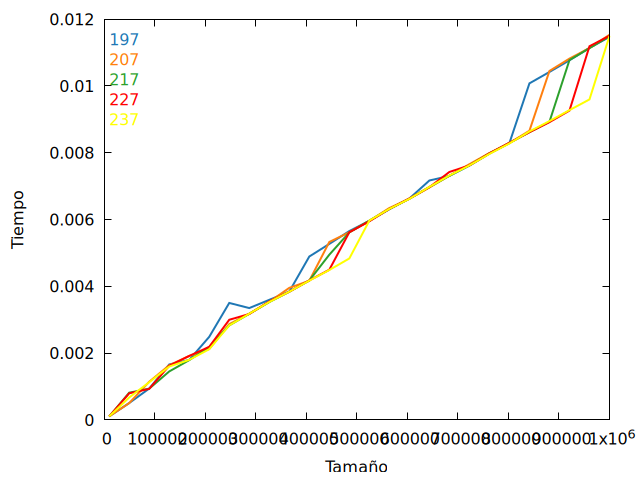
\includegraphics[scale = 0.4]{P1/UmmbralesTanteo.png}
        \caption{\centering Variación de eficiencia frente a variación de umbrales}
        
    \end{figure}\\
    Esta gráfica no tiene especial sentido, puesto que esta manera de calcular los umbrales de tanteo no la tiene, aún así, no es díficil comprender la gráfica, vemos que las 5 rectas se comportan de la misma forma, pero con un desfase de unas 10 unidades en el tamaño del problema, que es la variación de umbrales que hemos aplicado.
\newpage

\section{P2: Enlosar un espacio}

\subsection{Definición del problema}

    Queremos cubrir el suelo de una habitación cuadrada con baldosas en
    forma de ’ele’. En el suelo sabemos de la ubicación de un 
    sumidero que ocupa exactamente una loseta. Se pide
    encontrar la forma de colocar las losetas (sin romper ninguna) en
    nuestro suelo.
    
    Asumiremos que el suelo se representa como una matriz bidimensional
    A de tamaño $n \times n$,
    donde $n = 2k$ para algún $k >= 1$. La posición del sumidero la
    conocemos a priori por el par
    de valores $i$, $j$ con $0 \leq i, j \leq n - 1$. En nuestra matriz
    almacenaremos en la celda $A[i][j]$ el
    valor 0. Para cada baldosa que coloquemos en la matriz le asociaremos
    un identificador (entero)
    distinto. 
    
    Se pide diseñar una algoritmo que permita encontrar la forma de 
    rellenar el suelo (la matriz)
    de baldosas. 
    
    Por ejemplo, para una entrada del tipo
    \begin{verbatim}
    n = 2 
    i = 0 
    j = 0 
    Salida:
    0    1
    1    1
    n = 4
    i = 0
    j = 0
    Salida:
    0    3    2    2
    3    3    1    2
    4    1    1    5
    4    4    5    5
    \end{verbatim}

\subsection{Algoritmo específico} 

\subsubsection{Diseño e implementación} % Colaborativo

    Aunque la manera más directa y natural de resolver este problema sea utilizar la técnica divide y
    vencerás, existen otros diseños de algoritmos que resuelven el problema de forma aceptablemente
    natural. Uno de ellos es el algoritmo de completar cuadrados, cuya idea base es a partir
    de un cuadrado de tamaño $m \times m$, envolverlo con una L para formar un cuadrado
    de tamaño $2m \times 2m$. 

    En resumen, el algoritmo consiste en repetir este proceso desde el hueco $1 \times 1$
    que nos dan hasta completar el tablero $n \times n$ entero.

    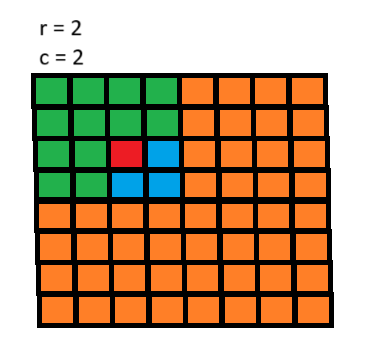
\includegraphics[width=0.4\textwidth]{P2/explicación0.png}

    Mirando la imagen superior, el algoritmo añadiría primero la L azul,
    envolviendo al sumidero rojo y completando un cuadrado $2 \times 2$ que 
    envuelve después con la L verde, completando un cuadrado $4 \times 4$,
    que finalmente envuelve con la L naranja, completando el tablero
    $8 \times 8$.

    La mayor complicación del algoritmo reside en ver en cada paso dónde y cómo colocar
    la L, además de cómo construir una L grande a partir de eles pequeñas.

    Para entenderlo, echemos un ojo a su implementación:

    \lstinputlisting[language=C++, firstline=93, lastline=112]{Codigos/P2/Lshapes_especifico.cpp}

    La función recibe como parámetros una matriz de enteros \texttt{v}, el lado \texttt{n} de dicha matriz,
    la posición \texttt{(r,c)} en la matriz, y un entero por referencia que será el número de losa
    que estemos poniendo (por facilitar la recursividad, aunque la función en sí no es recursiva). \\

    La función consta de un único bucle for con 6 líneas de cuerpo, y comienza calculando la
    orientación de la L que se va a colocar, siendo esta un entero del 0 al 3. El programa
    entiende que en el cuadrado
    \begin{verbatim}
        0   1
        2   3
    \end{verbatim}
    la orientación es la casilla que se deja libre al colocar la L. \\

    Por tanto, para calcular la orientación lo que se hace es dividir de 
    forma abstracta (\texttt{r/m} y \texttt{c/m})
    la matriz en cuadrados de tamaño $\texttt{m} \times \texttt{m}$ y ver en qué fila y
    columna está ese cuadrado dentro de uno de lado el doble (0 o 1) para
    finalmente coonvertir los dos dígitos binarios a un entero decimal
    del 0 al 3.

    Las siguientes dos líneas tienen como fin ajustar \texttt{i} y \texttt{j} a
    la esquina superior izquierda del cuadrado \texttt{m} $\times$ \texttt{m} que hemos
    construido.

    Las siguientes dos líneas tienn por objetivo ajustar \texttt{i} y \texttt{j} a la
    casilla exterior a la L que es adyacente a ambos brazos, es decir,
    la que se marca por x en los esquemas siguientes: \\
    \begin{verbatim}
        x   1           2   2   2   2
        1   1           2   2   2   2
                        2   2   x   .
                        2   2   .   .        
    \end{verbatim}
    Una vez se tiene esa casilla localizada y la orientación, la función
    \texttt{add\_slab\_m} se encarga de colocar la L de nivel m. Veamos
    el código de dicha función.

    \lstinputlisting[language=C++, firstline=21, lastline=70]{Codigos/P2/Lshapes_especifico.cpp}

    Esta función recibe la matriz \texttt{v}, el nivel de la L que vamos
    a añadir \texttt{m}, que no es más que el lado de cada uno de los 3
    cuadrados que la forman, la posición donde se inserta, que es la casilla
    adyacente a ambos brazos de la L, la orientación, que se define como
    se ha explicado previamente, y el número de losa básica que estamos 
    colocando.

    La función comienza calculando dos variables de incremento que servirán
    determinar donde y cómo colocar las baldosas, que valdrán 1 o -1 en
    función de la orientación de la L.

    A continuación se implementa el caso base \texttt{m == 1}, en el que
    como vemos a partir de la posición original \texttt{(i,j)} se añaden
    losas de tamaño 1 $\times$ 1 en las posiciones \texttt{(i,j+inc\_j)}, 
    \texttt{(i+inc\_i,j)} y \texttt{(i+inc\_i,j+inc\_j)}.

    Si no estamos en el caso base, utilizamos que podemos formar una L
    de nivel \texttt{m} con 4 eles de nivel \texttt{m/2} siguiendo el
    siguiente patrón: \\
    \begin{verbatim}
        .   .   3   3
        .   .   1   3
        2   1   1   4  
        2   2   4   4
    \end{verbatim}
    Donde cada terna de casillas con el mismo número forma una L de nivel
    \texttt{m/2} (recordemos que definimos el nivel de una L como el lado
    de cada uno de los tres cuadrados que la componen).
    Ahora la dificultad reside en calcular en que casilla y con qué
    orientación colocar cada una de las 4 eles.
    Primero nos damos cuenta de que la L interior y la exterior (1 y 4 en
    el esquema superior) tienen la misma orientación. Para las eles no
    adyacentes entre sí (la 2 y la 3 en el esquema), estudiamos cada caso
    por separado y vemos que en función de la orientación original, se
    obtienen los valores que se muestran en el esquema inferior para la
    orientación de la L 2 y la de la L 3 respectivamente: \\
    \begin{verbatim}
        0 --> 1 2
        1 --> 0 3
        2 --> 3 0
        3 --> 2 1
    \end{verbatim}
    De hecho se podría implementar con un switch tal y como está comentado
    en el código. No obstante las dos líneas para calcular orientation1
    y orientation2 dan un resultado equivalente (no sigue ningún fundamento
    matemático, simplemente surge de estudiar la casuística). 
    
    A continuación, escalamos los incrementos a la mitad del nivel de la L
    los incrementos para encontrar cada una de las posiciones de las 4 eles
    de nivel inferior.

    Para ver las posiciones donde insertar las eles de nivel inferior,
    nos apoyamos en el siguiente dibujo: \\

    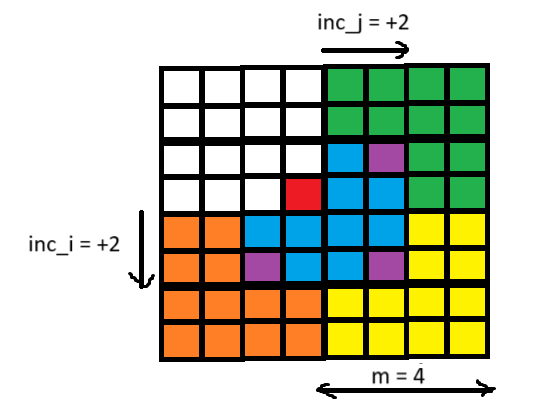
\includegraphics[width=0.7\textwidth]{P2/explicación1.png}

    Partiendo de la casilla roja \texttt{(i,j)} pretendemos insertar eles
    en las casillas moradas con sus respectivas orientaciones, además de en
    la casilla roja.

    La L azul no tiene mucho misterio, pues tiene la misma posición y orientación
    que la L original, solo que de nivel \texttt{m/2}. La L amarilla tampoco
    tiene mayor complicación, pues tiene la misma orientación pero insertada
    en la casilla \texttt{(i+inc\_i,j+inc\_j)}.

    La L naranja y la verde sí son más complicadas de calcular su posición,
    ya que aunque tengan el incremento calculado en una de sus coordenadas,
    también tienen el mismo incremento en la otra pero en sentido contrario
    y de una unidad menor.

    Y con esto termina la implementación del algoritmo, pues se añaden
    eles de nivel \texttt{m/2} recursivamente hasta llegar al caso base. \\
\subsubsection{Análisis de eficiencia} %    
\myparagraph{Eficiencia teórica} %

    Ahora procedemos a analizar la eficiencia teórica del algoritmo.
    En primer lugar observamos analizamos la eficiencia de la función
     \texttt{add\_slab\_m}.

    Si definimos la función $T$ que dado el tamaño del problema $m$, devuelve
    el tiempo que tarda en ejecutarse la función, como consta de 4 llamadas
    recursivas de tamaño $m/2$ entonces adopta la siguiente forma. \\

    \begin{equation} \label{eq:ef_dyv_p1}
    T\left(m\right) = \left\{ \begin{array}{lcc} 1 & m = 1  \\ \\ 
    4T\left(\frac{m}{2}\right) + 1 &  m > 1  \\ \end{array} \right. \hspace{10mm} \forall m = 2^k, k \in \N
    \end{equation} 

    Observamos que: 
\[
    T\left(m\right) = 4T\left(\frac{m}{2}\right)+1 = 4(4T\left(\frac{m}{4}\right)+1)+1= 
    4^2T\left(\frac{m}{2^2}\right)+1+4=4^kT\left(\frac{m}{2^k}\right)+\sum_{i=0}^k4^i \hspace{10mm}\forall k = 1\ ...\ \log_2\left(m\right)
\]
   %WAPO% 
   Desarrollando la suma de la progresión geométrica, nos queda:
\[
    T\left(m\right) = 4^kT\left(\frac{m}{2^k}\right)+\frac{4^{k+1}}{3} \hspace{10mm}\forall k = 1\ ...\ \log_2\left(m\right)
\]
    Y tomando $k=\log_2\left(m\right)$ obtenemos:
\[
    T\left(m\right) = 4^{\log_2\left(m\right)}T(1)+\frac{4^{\log_2\left(m\right)+1}}{3}=\frac{7}{3}m^2
\]    
    Por lo que concluimos que la eficiencia de la función \texttt{add\_slab\_m} es del orden $O(n^2)$ tomando como tamaño
    el lado de la matriz, si tomásemos como tamaño el número de elementos
    de la matriz sería del orden $O(n)$.

    Ahora volviendo a la función original, esta consta de un bucle
    \texttt{for} de $\log_2(n) - 1$ iteraciones en el que se llama a la función
    \texttt{add\_slab\_m} con todas las potencias de 2 desde 1 hasta $\nicefrac{n}{2}$.

    Si consideramos como tamaño del problema el número de elementos de la
    matriz, esta función es lineal como ya hemos visto. Así que la eficiencia
    de la función \texttt{fill\_L} será la suma de las potencias de 2 desde
    1 hasta $\nicefrac{n}{2}$, que es bien sabido que es la siguiente potencia de dos
    menos una unidad, es decir $n-1$, por tanto nuestra función tendrá
    nuevamente eficiencia $O(n)$ si consideramos como tamaño del problema
    el número de elementos de la matriz, y $O(n^2)$ si consideramos como
    tamaño del problema el lado de la matriz. \\

\myparagraph{Eficiencia empírica}

    A continuación procedemos al análisis de la eficiencia empírica. Para ello,
    hemos ejecutado el programa con todos los tamaños posibles en mi ordenador,
    es decir desde $n=2^0=1$ hasta $n=2^{14}=16384$, ya que la matriz resultante
    de la siguiente potencia sería de tamaño $n^2=2^{30}$ que ya no me cabe
    en memoria.

    Aquí están los tiempos de ejecución resultantes donde se ha considerado el
    tamaño del problema $n$ como el lado de la matriz:
    \begin{table}[H]
        \centering
    \begin{tabular}{|c|c|}
        \hline
        Tamaño(n) & Tiempo (seg) \\
        \hline
        1       & 2.1$\cdot 10^{-7}$ \\
        2       & 2.21$\cdot 10^{-7}$ \\
        4       & 5.82$\cdot 10^{-7}$ \\
        8       & 1.042$\cdot 10^{-6}$ \\
        16      & 3.516$\cdot 10^{-6}$ \\
        32      & 1.2954$\cdot 10^{-5}$ \\
        64      & 3.714$\cdot 10^{-5}$ \\
        128     & 0.000135897 \\
        256     & 0.000530396 \\
        512     & 0.00297852 \\
        1024    & 0.0131311 \\
        2048    & 0.0468183 \\
        4096    & 0.178777 \\
        8192    & 0.698544 \\
        16384   & 3.09681 \\
        \hline
    \end{tabular}
    \caption{\centering Tiempos obtenidos para el algoritmo DyV del problema 2}
    \end{table}

    \begin{figure}[H]
	\centering
	\begin{subfigure}{0.4\textwidth}
            \centering
            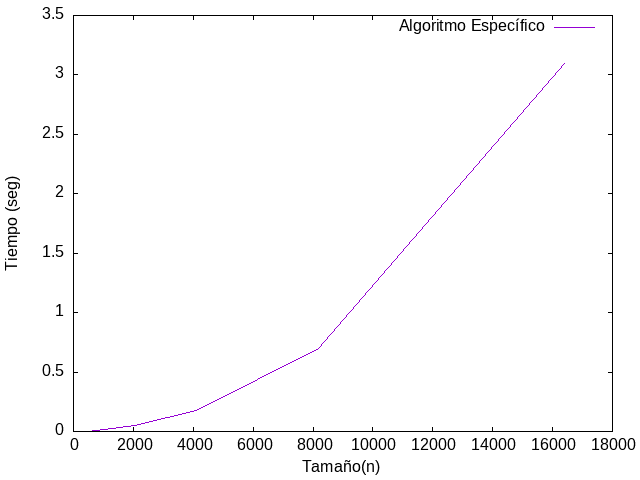
\includegraphics[scale = 0.40]{P2/lineas.png}
        \end{subfigure}	\hfill
	\begin{subfigure}{0.4\textwidth}
            \centering
            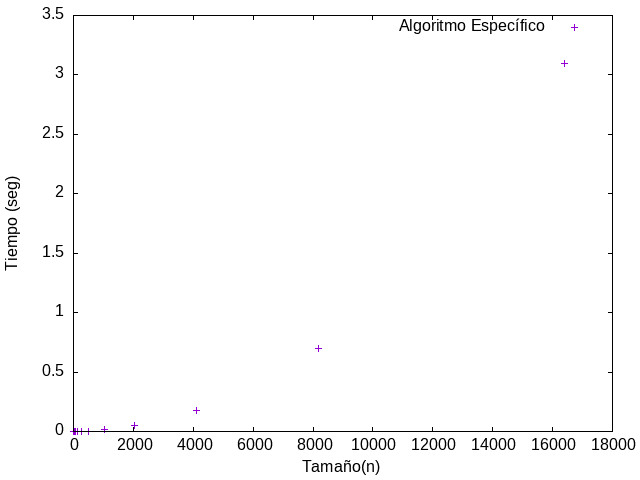
\includegraphics[scale = 0.40]{P2/puntos.png}
        \end{subfigure}
    \end{figure}

    Como el lado de la matriz siempre tiene que ser una potencia de 2, los puntos
    distan bastante entre sí. A pesar de ello, observamos que el crecimiento de
    los datos se asemeja a una función cuadrática. \\

\myparagraph{Eficiencia híbrida}

    En el análisis teórico hemos obtenido que la eficiencia del algoritmo
    es $O(n^2)$ si tomamos como tamaño $n$ el lado de la matriz cuadrada, y en
    el análisis empírico hemos visto que la relación tamaño-tiempo parece
    ser cuadrática.

    Veamos con más detalle que el análisis teórico se corresponde con la realidad,
    para ello, no tenemos más que realizar una regresión cuadrática de los puntos
    obtenidos con gnuplot, es decir, con una curva de la forma $f(x) = ax^2$. El
    resultado obtenido es:
\[
    f(x) = 1.14672 \cdot 10^{-8} \cdot x^2
\]
    \begin{figure}[H]
        \centering
        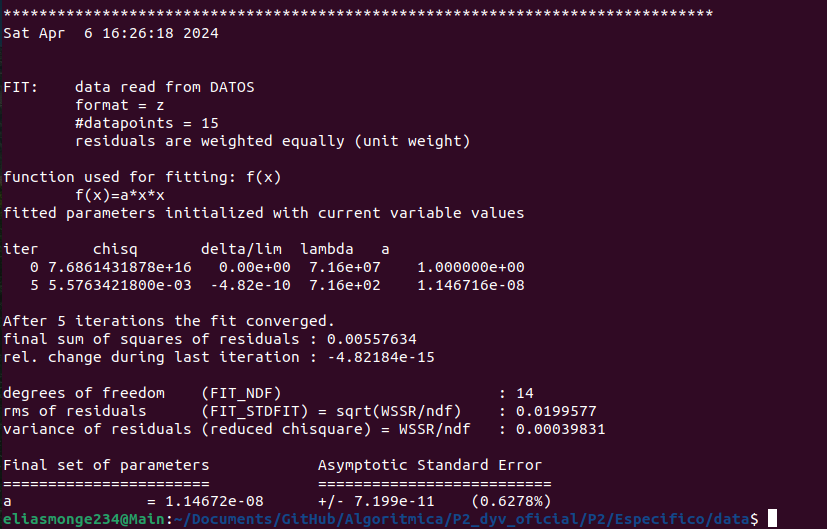
\includegraphics[scale=0.4]{P2/regresion_log.png} 
    \end{figure}

    \begin{figure}[H]
        \centering
        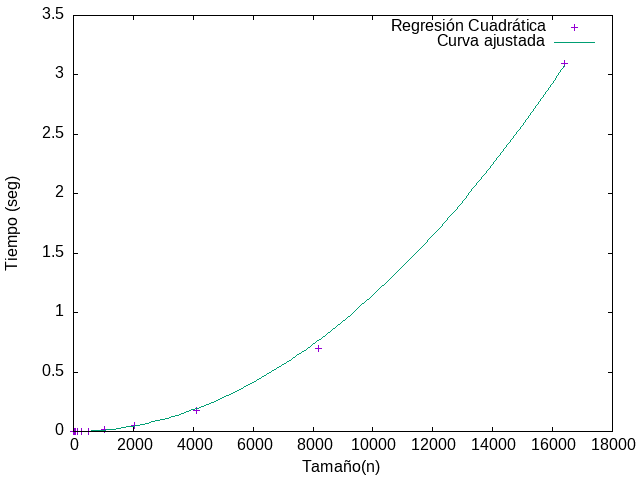
\includegraphics[scale=0.6]{P2/regresion.png} 
    \end{figure}

    Observamos que la varianza residual es casi nula, lo que significa un ajuste
    casi perfecto, respaldando nuestro resultado teórico. Esto se puede ver
    visualmente como que la curva pasa muy cerca de todos los puntos.

\subsection{Algoritmo divide y vencerás} 

\subsubsection{Diseño e implementación} % Colaborativo

    %% PD_OLGA: Pensaba que me tocaba a mí, he escrito algo. Te lo dejo 
    %% por si te sirve, sino eliminalo.

    %% PD_ELÏAS: No importa, muchas gracias :)
    
    Veamos el enfoque de Divide y Vencerás de este problema, que es la 
    forma más natural de resolverlo. En primer lugar,
    debemos ver cómo vamos a subdividir el problema en problemas de tamaño menor. \\ 
    
    Si dividimos la matriz en cuatro cuadrantes del mismo tamaño, que es posible porque $n$ es potencia de dos, podemos ver que el hueco siempre pertenece a algún cuadrante de tamaño $\frac{n}{2} \times \frac{n}{2}$. Para el resto de cuadrantes, que son tres, podemos colocar una baldosa L en el medio del tablero, de forma que no tape el cuadrante en el que estaba el hueco,
    pero sí los otros 3. \\
    
    Las 3 casillas pertenecen cada una a un cuadrante distinto, por lo
    que para rellenar cada uno de los 3 cuadrantes tenemos que rellenar todas
    sus casillas menos una, y tenemos una instancia del mismo problema de
    tamaño $\frac{n}{2}$. \\

    Siguiendo este proceso recursivamente hasta un caso base de tamaño
    $\text{UMBRAL}$ que podemos resolver con el algoritmo de completar cuadrados
    ya tenemos un algoritmo Divide y Vencerás para este problema. \\

    Para entenderlo mejor echemos un ojo a su implementación: \\

    \lstinputlisting[language=C++, firstline=118, lastline=119]{Codigos/P2/dyv.cpp}

    \lstinputlisting[language=C++, firstline=142, lastline=182]{Codigos/P2/dyv.cpp}

    En primer lugar describamos los parámetros que recibe. Recibe el lado
    del tablero \texttt{n}, la posición \texttt{(r,c)} del sumidero,
    la posición de la esquina superior izquierda de la matriz
    \texttt{(start\_row, start\_col)} para facilitar las llamadas recursivas,
    la matriz \texttt{v} y el número de losa \texttt{tile} que estamos
    colocando. \\

    Sigamos el flujo del programa. Si \texttt{n} es inferior o igual a un
    determinado umbral \texttt{\text{UMBRAL}} entonces enlosamos el tablero con el
    algoritmo específico de completar cuadrados. \\

    Si no, entonces entramos en un bucle \texttt{for} de cuatro iteraciones,
    que corresponderán a cada uno de los cuadrantes sobre los que vamos a
    llamar a la función recursivamente.
    
    Primero calculamos la posición inicial del cuadrante, a partir
    de dos arrays estáticos \texttt{sx} y \texttt{sy} según la iteración
    en la que estemos. \\

    Una vez tenemos la posición inicial, distinguimos el caso en el que
    el sumidero está en la submatriz obtenida, y llamamos a la función
    recursivamente con el mismo sumidero cambiando solo el tamaño y
    posiblemente la posición inicial. \\

    Si en el cuadrante en el que estamos no está el sumidero, entonces
    insertamos una casilla con valor \texttt{t} (correspondiente al número
    de losa original) y la tratamos como sumidero en la siguiente llamada
    recursiva. \\

    Para entenderlo visualmente, apoyémonos en el siguiente dibujo:
    \begin{figure}[H]
        \centering
        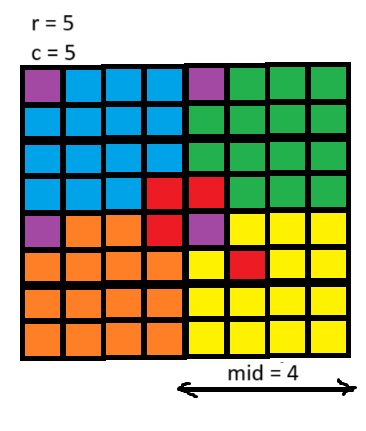
\includegraphics[width=0.35\textwidth]{P2/explicación2.png}
    \end{figure}

    Los colores azul, verde, naranja y amarillo rellenan los cuadrantes
    sobre los que se van a hacer llamadas recursivas, y la casilla morada
    dentro de cada uno la posición inicial que se calcula. Las casillas
    rojas dentro de cada cuadrante serían lo que se va a interpretar como
    sumidero en cada llamada recursiva, siendo el del cuadrante amarillo
    el sumidero original.

\subsubsection{Análisis de la eficiencia} %
\myparagraph{Eficiencia teórica} %

    Ahora vamos a estudiar cuál es la eficiencia teórica del algoritmo. Vemos que si definimos la función T que dado el tamaño del problema, $ m = n^{2}$, 
    devuelve el tiempo que tarda el programa en ejecutarse, entonces adopta la siguiente forma. 
    
    \begin{equation} \label{eq:ef_dyv_p1}
    T\left(m\right) = \left\{ \begin{array}{lcc} 1 & \sqrt{m}\leq \text{UMBRAL}  \\ \\ 
    4T\left(\frac{m}{4}\right) + 1 &  \sqrt{m} > \text{UMBRAL}  \\ \end{array} \right. \hspace{10mm} \forall n \in \N
    \end{equation}

    En el caso base, el tiempo está acotado por una constante luego podemos considerarlo en notación O grande como constante, por tanto es O(1), y en el caso general el código está compuesto en su totalidad por sentencias simples y un bucle que se ejecuta cuatro veces para repartir la tarea llamando cada vez a la función recursiva. Notese que para cada subllamada, el tamaño de entrada 
    es un cuarto del original.
    
    Supongamos que $\sqrt{m} > \text{UMBRAL}$  y efectuando el cambio de variable 
    $ 4^{t} = m \implies t = \log_{4}{m} = \log_{4}{n^2} $, calculamos : 

    \[ 
      T\left(m\right) = T\left(4^{t}\right) = 4 T\left(4^{t-1}\right) + 1 = 4 (4 T\left(4^{t-2}\right) + 1) + 1 = 4^{2} T\left(4^{t-2}\right) + 4 + 1 = 4^{3} T\left(4^{t-3}\right) + 4^{2} + 4 + 1 
    \]

    Tras aplicar k veces: 
    
    \[
      T\left(m\right)= 4^{k} T\left(4^{t-k}\right) + \sum_{i=0}^{k-1} 4^{i} 
    \]

    Si $ 4^{t-k} \leq \text{UMBRAL} \iff t - \log_{4}{\text{UMBRAL}} \leq k $ , entonces tenemos que si elegimos $\bar{k} = t - \log_{4}{\text{UMBRAL}} \implies T\left(4^{\bar{k}}\right) = 1$. Además, por la forma que hemos elegido t y teniendo en cuenta que n siempre es potencia de dos, podemos deducir que $\bar{k}$ con esta forma es un número entero, por tanto :
    
    \[
       T\left(4^{t}\right) = 4^{\bar{k}} T\left(4^{t-\bar{k}}\right) + \sum_{i=0}^{\bar{k}-1} 4^{i} =
       4^{\bar{k}} + \sum_{i=0}^{\bar{k}-1} 4^{i} =
       4^{\bar{k}} + \frac{1-4^{\bar{k}}}{3} = 
       \frac{1 + 2 \cdot 4^{\bar{k}}}{3} 
    \]
mathsf
    Deshaciendo el cambio de variable y teniendo en cuenta que 
    nos interesa calcular la eficiencia según la notación O grande: \\

    \[
        4^{\bar{k}} = 4^{t - \log_{4}{\text{UMBRAL}}} = 
        \frac{4^{t}}{\text{UMBRAL}} \iff 4^{\bar{k}} = 
        \frac{m}{\text{UMBRAL}}
    \]
    
    \[
        T\left(4^{t}\right) = \frac{1 + 2 \cdot 4^{\bar{k}}}{3} = 
        \frac{1 + 2 \cdot \frac{m}{\text{UMBRAL}}}{3} = T\left(m\right) \in O(m)
    \]

    NOTA: Como $m = n^{2}$, según qué consideremos 
    como tamaño de entrada en la análisis, cambia el orden de 
    eficiencia en el siguiente sentido: si consideramos como tamaño de entrada el número de elementos que tendrá la matriz, entonces, como hemos probado, el algoritmo es lineal. Sin embargo, si consideramos como tamaño de entrada el número de filas/columnas de la matriz, 
    entonces el algoritmo es cuadrático, puesto que $ O(m) = O(n^{2})$
    
\myparagraph{Eficiencia empírica}

    Con el algoritmo implementado y considerando como entrada 
    el número de filas/columnas de la matriz, al ejecutar el 
    programa con diferentes entradas obtenemos la siguiente
    tabla:
    \begin{table}[H]
        \centering
    \begin{tabular}{|c|l|}
        \hline
        Nº de filas & Tiempo (seg) \\
        \hline
        1       & $1.37 \cdot 10^{-7}$ \\
        2       & $2.11 \cdot 10^{-7}$ \\
        4       & $2.44 \cdot 10^{-7}$ \\
        8       & $3.80 \cdot 10^{-6}$ \\
        16      & $7.8 \cdot 10^{-6}$ \\
        32      & $2.42 \cdot 10^{-5}$ \\
        64      & $6.7  \cdot 10^{-5}$ \\
        128     & $0.000262055$ \\
        256     & $0.00104772$ \\
        512     & $0.00420025$ \\
        1024    & $0.0171024$ \\
        2048    & $0.0692816$ \\
        4096    & $0.267032$ \\
        8192    & $0.95623$ \\
        16384   & $3.53244$ \\
        \hline
    \end{tabular}
    \caption{\centering Tiempos obtenidos para el algoritmo DyV del problema 2}
    \end{table}

    Graficando los datos obtenidos obtenemos también: 

\begin{figure}[H]
    \begin{subfigure}{0.4\textwidth}
        \centering
        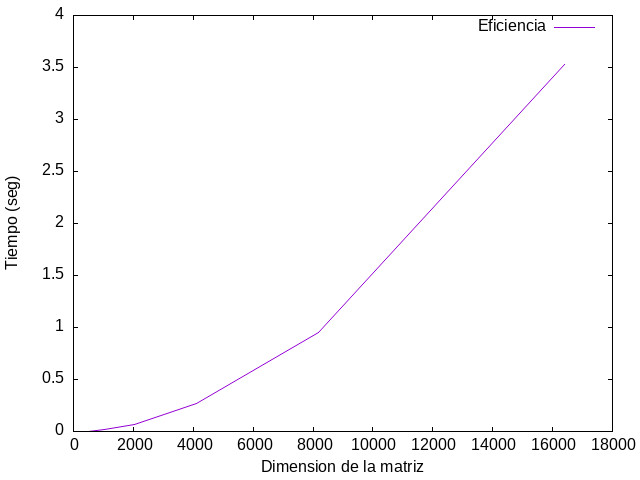
\includegraphics[scale = 0.40]{P2/L_Shape_DyV_lines.jpeg}
    \end{subfigure} \hfill
    \begin{subfigure}{0.4\textwidth}
        \centering
        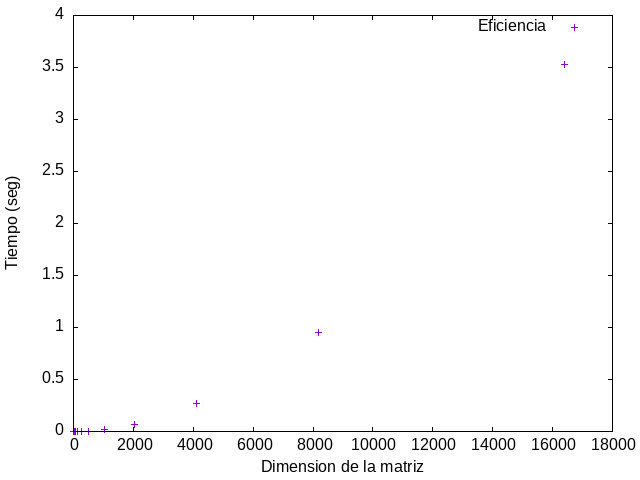
\includegraphics[scale = 0.40]{P2/L_Shape_DyV_puntos.jpeg}
    \end{subfigure}
\end{figure}


    Dado que se exige que el número de columnas/filas sean
    potencias de dos, podemos ver que los datos obtenidos están
    relativamente distados en la gráfica. Pero aun así, se puede apreciar que el crecimiento de los datos se parece a una curva cuadrática. 

\myparagraph{Eficiencia híbrida}

    Como teóricamente hemos obtenido que el algoritmo tiene una eficiencia de orden cuadrático, vamos a ajustarla con una curva de la forma $f(x) = a_0 x^{2}$. Veamos los resultados:

    \[
        f(x) = 1.32341\cdot10^{-8} x^{2}
    \]

    \begin{figure}[H]
        \centering
        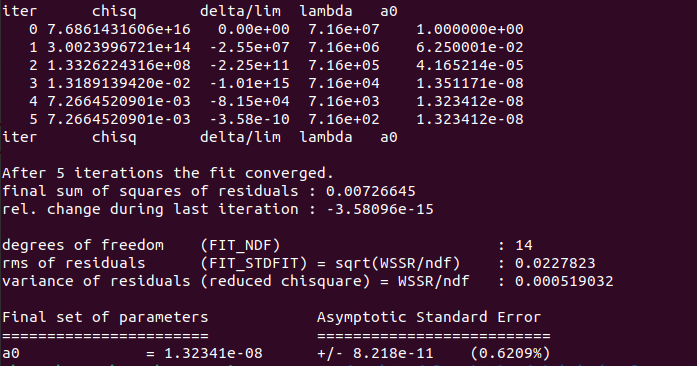
\includegraphics[scale=0.3]{P2/regresion_solo_DyV.png} 
    \end{figure}

    De los resultados podemos ver que la varianza residual es casi nula, lo cual quiere decir que nuestro ajuste se ajusta a nuestros datos casi a la perfección -- verificando los resultados teóricos que afirman que la eficiencia del algoritmo es de $O(n^{2})$. 

    Veamos la curva de regresión graficada con los datos:
    
    \begin{figure}[H]
        \centering
        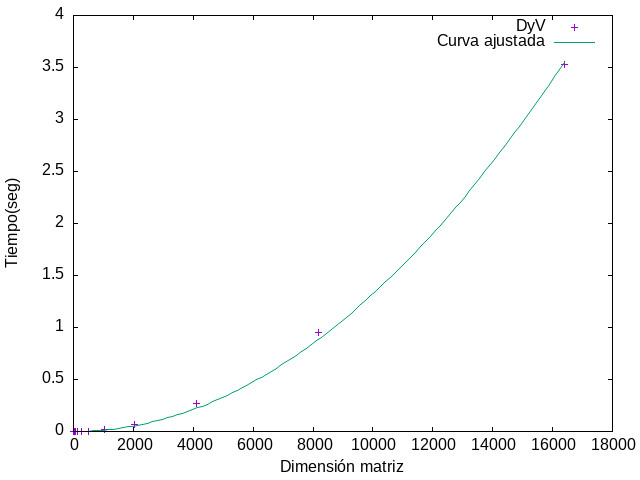
\includegraphics[scale = 0.5]{P2/Salida_ajustada1.jpeg}
    \end{figure}

    Conclusión: En efecto, los resultados empíricos se ajustan a los teóricos.
    
\subsubsection{Cálculo de umbrales} %

    En esta sección calcularemos los umbrales teórico, óptimo y de tanteo,
    para posteriormente compararlos gráficamente. \\

    \myparagraph{Umbral teórico}

    Para el cálculo del umbral teórico, planteamos la ecuación del algoritmo
    específico tal cual ($h(n)=n^2$), la aplicamos en el primer nivel de recurrencia y resolvemos la ecuación (no recurrente):

    \begin{equation} \label{eq:ef_dyv_p1}
    T(n) = \left\{ \begin{array}{lcc} n^2 & n \leq \text{UMBRAL}  \\ \\ 
    4T\left(\nicefrac{n}{2}\right) + 1 &  n > \text{UMBRAL}  \\ \end{array} \right. \hspace{10mm} \forall n \in \N
    \end{equation}

    Entonces nos queda: 
\[
    n^2=4\frac{n^2}{4}+1 \iff 0=1
\]
    Con lo que concluimos que no podemos calcular el umbral teórico
    para este algoritmo. Este resultado se da por tener ambos algoritmos
    el mismo orden de eficiencia, y es una prueba más de que el umbral teórico
    es meramente indicativo. \\

    \myparagraph{Umbral óptimo} 

    Para el cálculo el umbral óptimo, planteamos la función del algoritmo
    específico obtenida en la eficiencia híbrida ($h(n) = 1.14672 \cdot 10^{-8} \cdot n^2$), la aplicamos en el primer nivel de recurrencia y resolvemos la ecuación (no recurrente):

    \begin{equation} \label{eq:ef_dyv_p1}
    T(n) = \left\{ \begin{array}{lcc} n^2 & n \leq \text{UMBRAL}  \\ \\ 
    4T\left(\nicefrac{n}{2}\right) + 1 &  n > \text{UMBRAL}  \\ \end{array} \right. \hspace{10mm} \forall n \in \N
    \end{equation}

    Entonces nos queda:

    $$
    1.14672 \cdot 10^{-8} \cdot n^2=4\frac{1.14672 \cdot 10^{-8} \cdot n^2}{4}+1 \iff 0=1
    $$

    Al igual que con el umbral teórico, vemos que no tiene sentido resolver esta ecuación dado que ambos algoritmos tienen el mismo orden de eficiencia, y por tanto de forma teórica no tiene sentido tratar de calcular ningún umbral.

    \myparagraph{Umbral empírico}

    Al tener ambos códigos la misma eficiencia, como hemos visto, no tienen mucho
    sentido los cálculos teóricos para el umbral, por lo que tomaremos ahora
    un enfoque empírico para el cálculo del umbral.

    Para ello representamos la ejecución de ambos algoritmos (el divide y vencerás con
    umbral=0) y vemos a partir de qué tamaño $n$ es más rápido (menor tiempo) el
    algoritmo divide y vencerás:

    \begin{figure}[H]
        \centering
        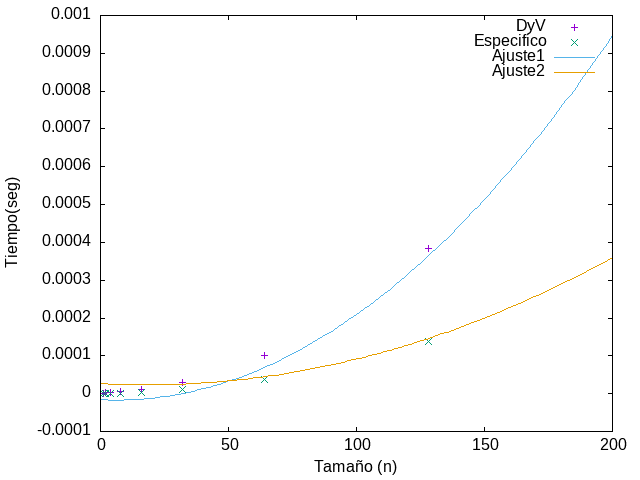
\includegraphics[scale=0.7]{P2/u1.png} 
    \end{figure}

    Como vemos, la gráfica representa la situación opuesta a la que esperábamos,
    ya que la gráfica amarilla del algoritmo específico queda por debajo de la 
    del algoritmo divide y vencerás, algo que va completamente en contra de la
    filosofía del algoritmo. Esto ocurre ya que el algoritmo específico, aunque
    sea de la misma eficiencia que el algoritmo divide y vencerás, tiene mejores
    constantes ocultas que el algoritmo divide y vencerás, y por tanto es más
    eficiente. No obstante podemos destacar el tramo en el que el algoritmo divide
    y vencerás es más eficiente, que es aproximadamente entre 0 y 50.

    \myparagraph{Umbral de tanteo}

    Aunque no hayamos obtenido un umbral empírico como tal, vamos a tratar
    de comparar diferentes umbrales en cuanto a tiempos de ejecución para ver
    qué ocurre. En principio podríamos suponer que a mayor umbral mayor será
    el tiempo de ejecución pues se delega más trabajo en el algoritmo más eficiente.
    Como los tamaños del problema son potencias de 2, cogeremos umbrales de
    tamaño potencia de 2.
    El resultado para los umbrales 2, 16, 128, 512, 2048 y 16384 es el siguiente:
    
    \begin{figure}[H]
        \centering
        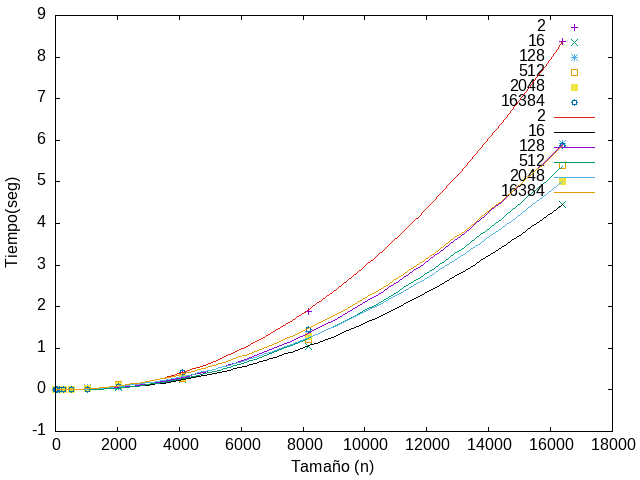
\includegraphics[scale=0.7]{P2/Salida_comparativa1.png} 
    \end{figure}

    Como vemos los tiempos son relativamente similares a excepción del caso
    $\text{UMBRAL}=2$ que sí que es cierto que es más lento que el resto. También llama la
    atención que no se verifica nuestra hipótesis de que a mayor umbral menor tiempo,
    pues a pesar de que $\text{UMBRAL}=16384$ es más rápido que la mayoría, $\text{UMBRAL}=16$
    es el más rápido de todos.

    Podríamos pensar que entonces el umbral óptimo se hallaría cerca del 16. Probemos
    con umbrales cercanos:

    \begin{figure}[H]
        \centering
        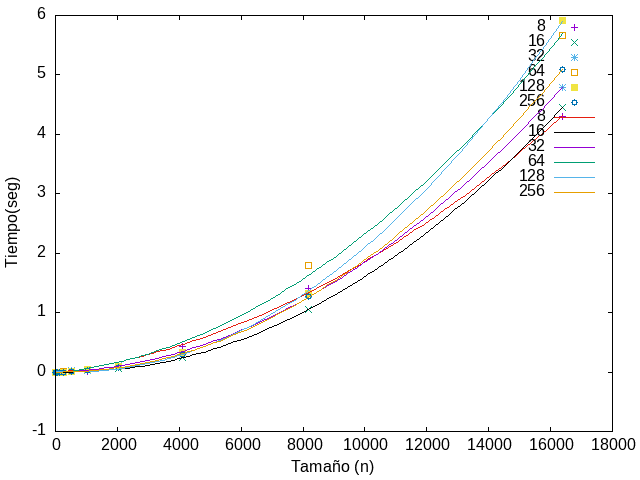
\includegraphics[scale=0.7]{P2/Salida_comparativa2.png} 
    \end{figure}

    En efecto, en orden de velocidad tendríamos primero el 8, después el 16,
    y después el 32, cercanos al 16. Curiosamente el siguiente sería el 256
    mostrando que aunque no sea óptimo, es bueno coger umbrales grandes
    delegando gran parte del trabajo en el algoritmo específico.

    \myparagraph{Conclusión}

    Como conclusión tendríamos que el cálculo de umbrales no tiene mucho
    sentido cuando dos algoritmos tienen la misma eficiencia, al menos a
    nivel teórico. No obstante por tanteo descubrimos que el umbral ideal
    es $\text{UMBRAL}=8$, aunque también son buenos los umbrales grandes al ser
    más rápido el algoritmo específico.
    

\newpage
\section{P3: Problema del viajante de comercio}

\subsection{Definición del problema}


Tenemos un conjunto de $n$ ciudades (puntos en un plano),
cada una definida por las coordenadas en el mapa $(x_i, y_i)$,
con $i = 1,\ ...\ , n$. La distancia entre dos ciudades viene
dada por la distancia euclídea entre sus coordenadas.
\[
dist((x_1, y_1),(x_2, y_2)) = \sqrt{(x_1 - x_2)^2 + (y_1 - y_2)^2}
\]

El problema de viajante de comercio consiste en encontrar el
orden en el que un viajante, partiendo de la ciudad de origen
(por ejemplo $(x_1, y_1)$) pase por todas y cada una de las ciudades
una única vez, para volver a la ciudad de partida, formando un ciclo.

El costo del ciclo será la suma de las distancias que hay entre todas las ciudades consecutivas.

El problema original del viajante de comercio consiste en encontrar el ciclo de costo mínimo entre todas las posibilidades existentes.

Aunque este problema es NP-Difícil y por tanto no podemos esperar
encontrar una solución óptima al mismo, lo que se pretende en esta
práctica es utilizar la estrategia del divide y vencerás
para encontrar una solución aproximada que puede ser de utilidad en
situaciones como las que se plantea en este problema.

\subsubsection{struct City}

Para resolver este problema con mayor comodidad y facilitar la modularización y legibilidad del código, se ha hecho uso de una  $struct$ $City$ para representar las ciudades del problema.
\lstinputlisting[language=C++, firstline=5,lastline=7]{Codigos/P3/City.h}
Se ha definido también una constante $INF$ para representar un valor de distancia imposible mayor que cualquier otro de los que pueda haber dentro del problema.
\lstinputlisting[language=C++, firstline=7,lastline=9]{Codigos/P3/City.h}
%\lstinputlisting[language=C++, firstline=14,lastline=62]{Codigos/P3/City.h}

La $struct$ $City$ representa las ciudades del problema mediante sus coordenadas $(x,y)$.\\
\lstinputlisting[language=C++, firstline=14,lastline=16]{Codigos/P3/City.h}
Además implementa la función $dist$ que calcula la distancia euclídea de una ciudad a otra y tiene sobrecargado el operador $-$ para este mismo propósito.
\lstinputlisting[language=C++, firstline=21,lastline=30]{Codigos/P3/City.h}

El operador $<$ también ha sido sobrecargado puesto que en nuestros algoritmos nos valimos de ordenar las ciudades respectod el eje $x$ para dar con soluciones más óptimas y eficientes.

\lstinputlisting[language=C++, firstline=32,lastline=41]{Codigos/P3/City.h}

Por último se han sobrecargado los operadores distinto ($!=$) y igual ($==$) por comodidad a la hora de trabajar con $City$ y los operadores de entrada ($>>$) y salida ($<<$) para facilitar la lectura y escrituda de datos.

\lstinputlisting[language=C++, firstline=43,lastline=60]{Codigos/P3/City.h}

Para finalizar, se ha implementado la función $printCycle()$ la cual recibe como parámetros el orden de los índices de las ciudades, la ciudad de origin y un array con las ciudades e imprime las ciudades empezando y acabando en la ciudad de origen en el orden indicado. Esto se ha hecho para facilitar la impresión de ciudades en el orden correcto teniendo en cuenta que el array de ciudades original ha sido ordenado.

\lstinputlisting[language=C++, firstline=101,lastline=111]{Codigos/P3/City.h}

\subsection{Algoritmo específico} 

\subsubsection{Diseño e implementación} % Colaborativo
\myparagraph{Diseño}
El algoritmo específico elegido para resolver el problema del viajante de comercio ha sido uno que nos de la solución óptima al problema, a costa de un gran coste de eficiencia. La única forma conocida de dar con la solución óptima al problema es probar todos los ciclos posibles y quedarnos con el ciclo óptimo de todos ellos, es decir, resolver el problema mediante fuerza bruta. No obstante, hemos introducido pequeñas mejoras que aunque no afectan a la complejidad del algoritmo en el caso general (el orden de eficiencia sigue siendo el mismo) si que mejoran los tiempos obtenidos en media.
\newline
\newline
Para explorar todos los ciclos posibles, partimos de la ciudad de origen, y de ahí vamos a la primera ciudad que no hayamos visitado. Procedemos a visitarla añadiendola a nuestro ciclo actual y acumulando la distancia de la ciudad origen a esta. Una vez hecho eso repetimos el proceso solo que desde la última ciudad visitada, así hasta a ver visitado todas las ciudades en cuyo caso ya tenemos uno de los ciclos posibles. Una vez completada la investigación de este ciclo probamos a visitar la segunda ciudad posible desde la última ciudad visitada y así sucesivamente. Es decir, si tenemos en total $n = 4$ ciudades numeradas del 0 al 3, con la ciudad de origen el 0, partimos de la ciudad 0. Como no hemos visitada ningún otra ciudad, visitamos la ciudad 1, después la 2 y por último la 3. Una vez completado el ciclo, volvemos a la ciudad 2 y vemos si podemos visitar otra ciudad distinta a la 3. Como no es el caso, volvemos a estar en la ciudad 1, y en este caso en vez de visitar la ciudad 2 visitamos la 3 y así sucesivamente.
\newline 
Todos los caminos recorridos pueden verse en la figura \ref{fig:permutacion} donde cada flecha representa una llamada a la función a visitar la ciudad apuntada por la flecha con las ciudades previas a la flecha visitadas.
\newline
\begin{figure}[!hbt]
    \centering
    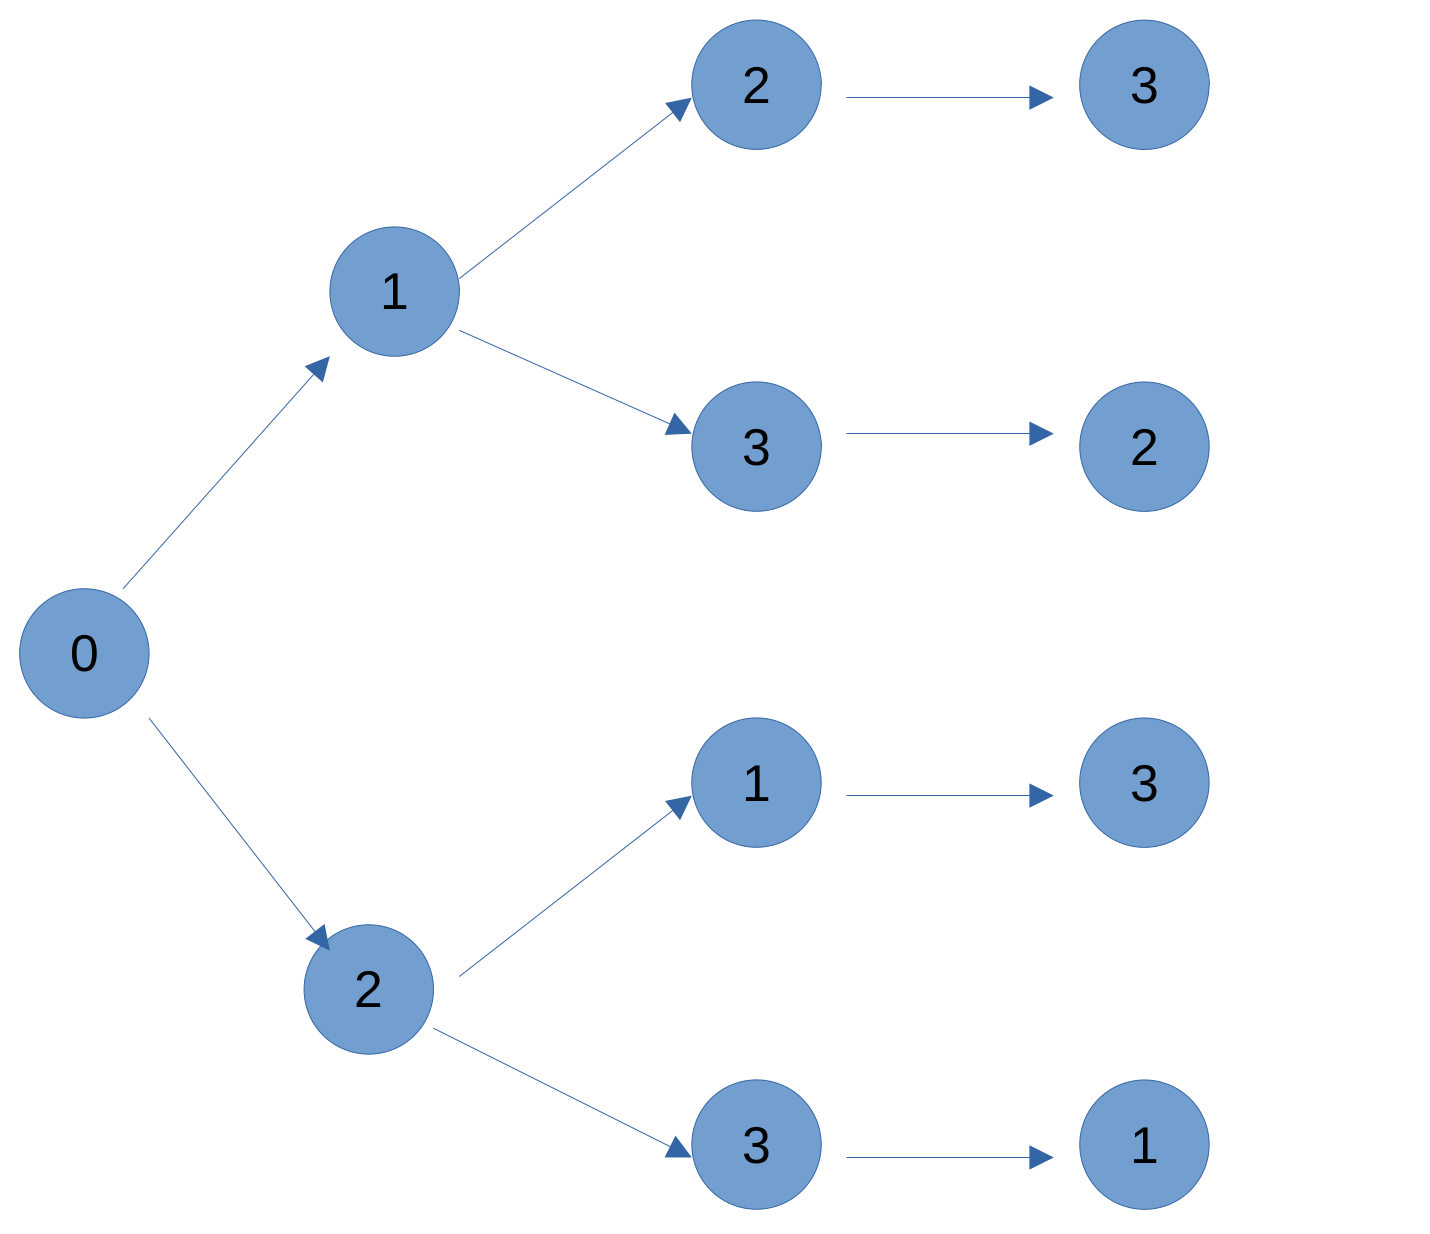
\includegraphics[scale=0.2]{P3/Prosa/permutacion.png}
    \caption{\centering Todos los caminos posibles para n = 4}
    \label{fig:permutacion}
\end{figure}
La mejora implementada consiste en a medida que se va calculando el coste de un ciclo, es decir, a medida que se van visitando ciudades y acumulando las distancias recorridas, en el momento en el que la distancia recorrida actual es mayor o igual que el coste de nuestro mejor ciclo hasta la fecha, abandonamos ese camino por completo dado que no nos va a proporcionar una solución mejor a la que ya tenemos puesto que todas las distancias son estrictamente positivas.
\newline
Veamoslo con un ejemplo. En la figura \ref{fig:arbol_coste} podemos ver el arbol de recorridos para $n=4$ ciudades con unas distancias de ejemplo (las distancias escogidas nos son reales dado que no cumplen las propiedades geométricas de la distancia euclídea, no obstante sirven para ejemplificar el algoritmo). En la figura \ref{fig:arbol_branch_bound} podemos ver los recorridos que haría el algoritmo de todos los que hay, empleando que el primer recorrido que hace es el de las ciudades en orden y que en el momento en el que ir a una ciudad le supone que lleva una distancia mayor al coste mínimo actual no la visita.
\newline
\begin{figure}[!hbt]
    \centering
    \begin{subfigure}{0.4\textwidth}
        \centering
        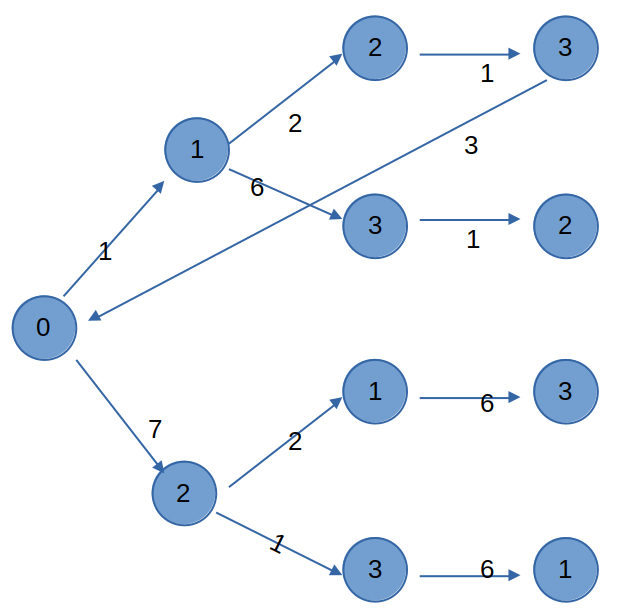
\includegraphics[width=\textwidth]{P3/Prosa/arbol_coste.png}
        \caption{\centering Todos los caminos con sus costes}
        \label{fig:arbol_coste}
    \end{subfigure}
    \hfill
    \begin{subfigure}{0.4\textwidth}
        \centering
        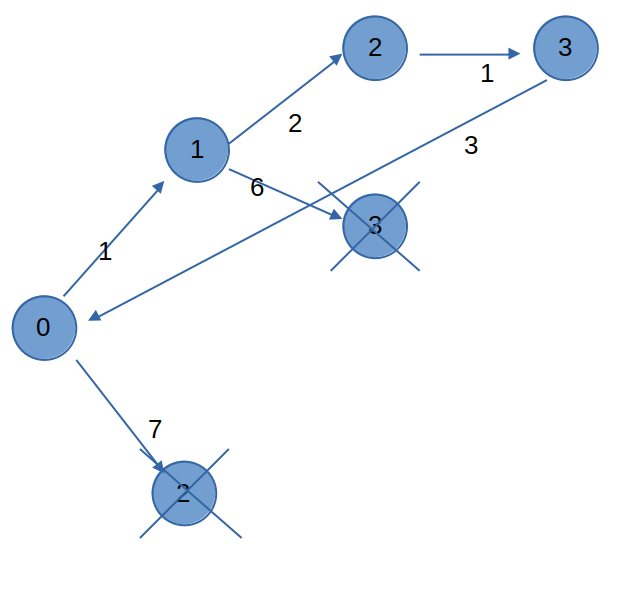
\includegraphics[width=\textwidth]{P3/Prosa/arbol_branch_bound.png}
        \caption{\centering Caminos recorridos por el algoritmo}
        \label{fig:arbol_branch_bound}
    \end{subfigure}
\end{figure}
En el ejemplo podemos ver como el primer camino recorrido tiene coste 7, y por tanto cuando el algoritmo detecta que ir a una ciudad le supone ya un coste 7 o superior abandona el camino "podando esa rama" y pasa a la siguiente opción. De esa forma los caminos (llamadas a la función) recorridos en la figura \ref{fig:arbol_branch_bound} son muchos menos (muchas menos llamadas recursivas) que en la figura \ref{fig:arbol_coste}.
\newline
Como hemos podido observar, la mejora en eficiencia se aprovecha más cuanto menor es el coste del primer ciclo explorado, el cual siempre es el array de ciudades en orden. Por este motivo hemos optado por ordenar previamente el array para garantizar que el primer ciclo explorado es "relativamente" bueno en comparación al todos los demás ciclos posibles.
\myparagraph{Implementación}
Para implementar el algoritmo hemos empleado una función recursiva que tiene como parámetros:
\begin{itemize}
    \item $n$: número total de ciudades a visitar
    \item $prev$: el índice de la última ciudad visitada
    \item $homeind$: el índice de la ciudad de origen
    \item $cnt$: número de ciudades visitadas
    \item $v$: el array con las ciudades
    \item $visited$: un array que indica si hemos visitado la ciudad $i$ o no
    \item $dist$: distancia actual
    \item $bestdist$: mejor distancia encontrada hasta ahora (inicialmente se pone a $INF$)
    \item $curcycle$: camino recorrido hasta ahora
    \item $bestcycle$: mejor ciclo encontrado hasta ahora
\end{itemize}

\lstinputlisting[language=C++, firstline=18,lastline=18]{Codigos/P3/especifico.cpp}

\begin{itemize}
    \item \textbf{Caso base:} 
    \newline
    Consiste en haber visitado ya todas las ciudades ($n-1$) y por tanto solo queda añadir la distancia de la última ciudad visitada a la ciudad de origen para tener el coste del ciclo total. Una vez hecho eso comprobamos si este coste es menor que el de nuestro ciclo más óptimo hasta la fecha y si es así lo actualizamos.

    \lstinputlisting[language=C++, firstline=19,lastline=30]{Codigos/P3/especifico.cpp}

    \item \textbf{Caso general:} \\
    Si todavía no hemos visitado todas las ciudades, entonces iteramos por todas ellas hasta dar con una que no hayamos visitado todavía, en cuyo caso la visitamos marcándola como visitada, añadiendola a nuestro camino actual y sumando la distancia de la ciudad elegida a nuestra última ciudad visitada a nuestra distancia actual. 
    \lstinputlisting[language=C++, firstline=32,lastline=38]{Codigos/P3/especifico.cpp}
    La mejora introducida es la siguiente: normalmente, si quisieramos explorar todos ciclos posibles, llamaríamos a nuestra función recurrentemente con la nueva ciudad visitada. No obstante, como todas las distancias son positivas, sabemos que si nuestra distancia actual ($dist$) es mayor o igual que nuestra distancia más óptima hasta ahora, tenemos garantizado que llendo por este camino no podremos mejorar nuestra mínima hasta el momento, por tanto seguir ese camino no nos aporta nueva información y nos hace perder un valioso tiempo. Es por eso que si la distancia actual es peor que el coste de nuestro ciclo mínimo actual, no la visitamos y simplemente pasamos a probar con la siguiente ciudad posible. \\
    En caso contrario, si que llamamos a nuestra función recursiva con una ciudad más visitada para explorar todos los posibles caminos con las ciudades que nos faltan por visitar. Una vez completado esto, volvemos a marcar la ciudad como no visitada y a eliminarla del camino, y pasamos a probar a visitar la siguiente ciudad posible.
    \lstinputlisting[language=C++, firstline=39,lastline=51]{Codigos/P3/especifico.cpp}
    Es fácil ver, que nuestra mejora será más efectiva cuanto menor sea el coste del primer ciclo, puesto que así será más probable que explorar otros caminos sea innecesario. Por ello, antes de llamar a la función, ordenamos el array de las ciudades respecto del eje $x$, ya que el primer ciclo explorado de todos es el array en orden, y las ciudades ordenadas por el eje $x$ aunque no sean el ciclo óptimo nos garantizan que las ciudades consecutivas estarán más o menos cerca entre sí y por tanto no será una solución del todo "mala".
    \lstinputlisting[language=C++, firstline=67,lastline=67]{Codigos/P3/especifico.cpp}
\end{itemize}

\subsubsection{Análisis de eficiencia} %
\myparagraph{Eficiencia teórica}
De la misma forma que los casos anteriores, definimos la función $T:\mathbb{N} \to \mathbb{R} $ que toma un número natural n como tamaño 
de la entrada (número de ciudades para las que calcular el camino mínimo necesario para pasar por cada una de ellas) y nos retorna 
el número de operaciones que necestiamos realizar (en el peor caso) para obtener un resultado para ese tamaño usando un enfoque de fuerza brutal. El código que implementa la solución ya explicada es el siguiente:

\lstinputlisting[language=C++, firstline=7, lastline=41]{Codigos/P3/dyv.cpp}


Observando el código es claro que, en el peor de los casos
(que se efectúen todas las iteraciones del bucle \textit{for} posibles en cada una de las llamadas recursivas) nos encontramos con
que para resolver el problema de tamaño $n$ se hacen n llamadas 
a recursivas sobre problemas de tamaño $n-1$, luego:

\begin{equation} 
T(n) = \left\{ \begin{array}{lcc} 1 & n = 0  \\ \\ 
n\cdot T(n-1) + 1 &  n > 0 \\ \end{array} \right. \hspace{10mm} \forall n \in \N
\end{equation}

Demos un esquema de la demostración por inducción del siguiente
hecho:
\[
T(n) = n!\cdot \sum_{k=0}^{n} \frac{1}{k!}
\] 

\begin{proof}
Caso $n=0$:
\[
1 = T(0) = 0! \cdot \sum_{k=0}^{0} \frac{1}{k!}
\] 

Caso $n\ge 1$: Suponemos $T(n-1)$ se tiene.\newline


\[
T(n) = n \cdot T(n-1) + 1 = 1 +  n\cdot(n-1)!\cdot \sum_{k=0}^{n-1} \frac{1}{k!} \\
= n!  \cdot (\sum_{k=0}^{n-1} \frac{1}{k!} + \frac{1}{n!} )\\
= n!\cdot \sum_{k=0}^{n} \frac{1}{k!} \\
\] 
\end{proof}

Por tanto, tenemos de manera clara (por la regla del máximo) que
la eficiencia de este algoritmo es del orden $O\left( n! \right)$

\myparagraph{Eficiencia empírica}
Usamos de manera análoga a los casos ya vistos en anteriores ocasiones la herramienta de gnuplot para representar gráficamente
los resultados de tiempos de ejecución obtenidos para distintos tamaños de entrada del problema. Tomamos un rango de tamaño de 1 a 14, pues al ser factorial crece súmamente rápido y el tiempo de ejecución es inasumbible para mi máquina con tamaños superiores a ese.

Los datos obtenidos son los siguientes:

\begin{figure}[H]
    \begin{subfigure}{0.4\textwidth}
        \centering
        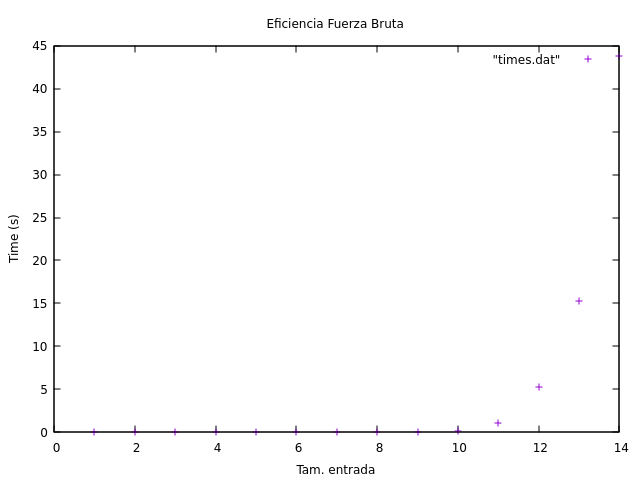
\includegraphics[scale = 0.40]{P3/fb_points.png}
    \end{subfigure} \hfill
    \begin{subfigure}{0.4\textwidth}
        \centering
        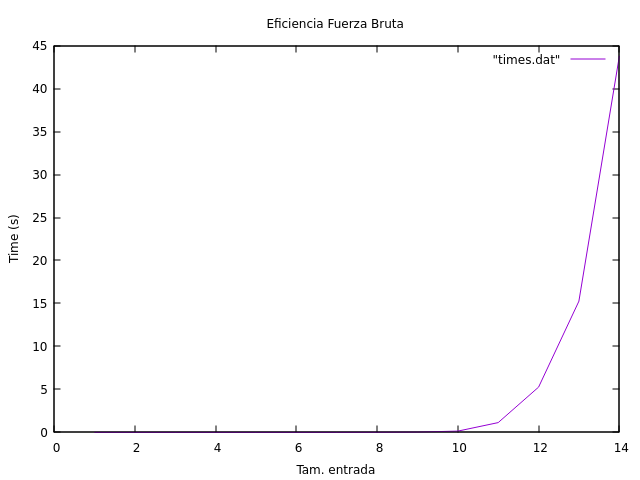
\includegraphics[scale = 0.40]{P3/fb_lin.png}
    \end{subfigure}
\end{figure}
\newpage
\myparagraph{Eficiencia híbrida}
Para hacer un ajuste, intentamos poner nuestros resultados como
una función $f(x) = c_{0} \cdot n!$. El resultado obtenido usando \textit{gnuplot} es el siguiente:
\newline
\begin{figure}[H]
    \centering
    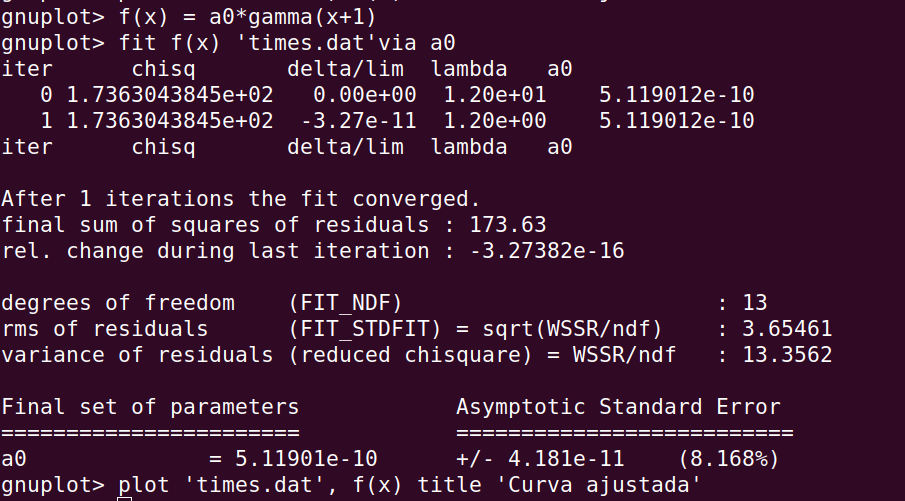
\includegraphics[scale = 0.4]{P3/datos_gnu_plot.png}
    \caption{\centering Comandos usados en gnuplot}
    \label{fig:comandos_gnuplot_bf}
\end{figure}\hfill
\begin{figure}[H]
    \centering
    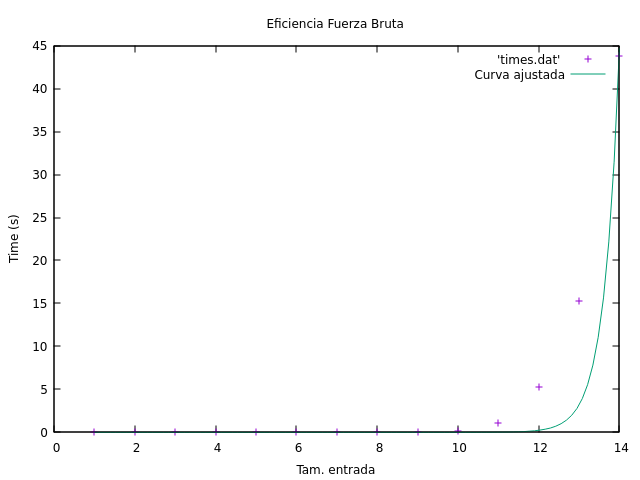
\includegraphics[scale = 0.4]{P3/fb_ajsute_gamma.png}
    \caption{\centering Función de ajuste $5.110\cdot10^{-10} \cdot fact(n)$}
    \label{fig:comandos_gnuplot_bf}
\end{figure}

Nótese que, naturalmente, no hemos utilizado la función 
factorial (que está definida en los naturales) sino una extensión
suya a la los reales positivos, la función Gamma:

\[
\Gamma(z) = \int_{0}^{\infty} t^{z-1}e^{-t}\,dt \quad \forall z \in \mathbb{R^{+}}
\]
Pues se puede demostrar que:
\[
\Gamma(n+1) = n! \qquad \forall n \in \mathbb{N}
\]


\subsection{Algoritmo divide y vencerás}

\subsubsection{Diseño e implementación} % Colaborativo
\myparagraph{Diseño}
A la hora de abordar la implementación divide y vencerás de este problema, hemos tenido en cuenta que se trata de un problema NP-Difícil y por tanto no se puede obtener su solución óptima en tiempo polinómico con nuestros ordenadores actuales (se puede calcular en tiempo polinómico con una máquina de Turing no determinista). Por tanto, hemos optado por un algoritmo que de una solución \textbf{aproximada}.
\newline
Tras probar distintos enfoques, hemos concluido que la forma más eficiente y que da la solución más óptima (el error respecto a la solución óptima real es menor) de aplicar divide y vencerás a este problema es la siguiente: 
\begin{enumerate}
    \item Ordenar las ciudades respecto a su coordenada $x$
    \item Partir el array ordenado por la mitad, diviendolo en dos subgrupos del mismo tamaño (aprox) cuyos integrantes se encuentran cerca los unos de los otros (respecto al eje X)
    \item Una vez obtenida la solución para ambos grupos, gracias a que sabemos por donde partimos el array, conocemos las dos ciudades más próximas respecto a eje X entre ambos ciclos. Para cada una, se escoge una de sus ciudades adyadcentes, en particular la que este más centrada respecto al eje X.
    \item Ya seleccionadas ambas parejas, se separan y se une cada uno de ellas con un miembro de la pareja del otro ciclo. Hay dos formas, se realiza de la que sea más eficiente.
    \begin{figure}[H]
    \centering
    \begin{subfigure}[b]{0.3\textwidth}
        \centering
        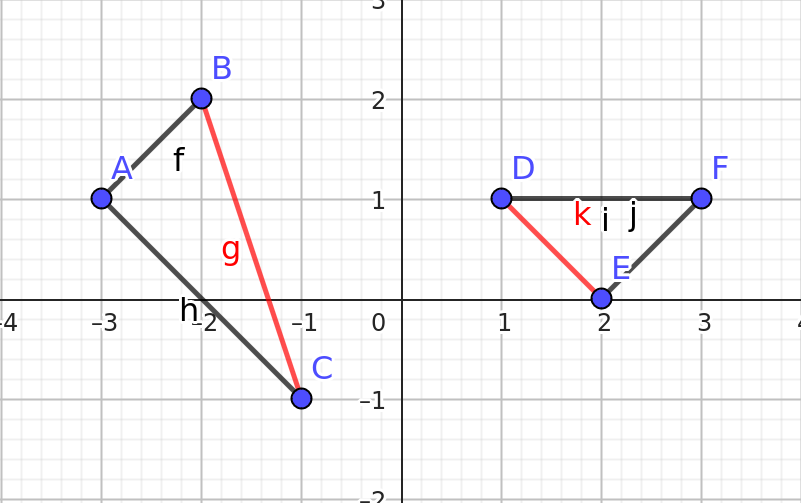
\includegraphics[width=\textwidth]{P3/Prosa/ej_unir0.png}
        \caption{\centering Estado inicial}
        \label{fig:p3_ejemplo}
    \end{subfigure}
    \hfill
    \begin{subfigure}[b]{0.3\textwidth}
        \centering
        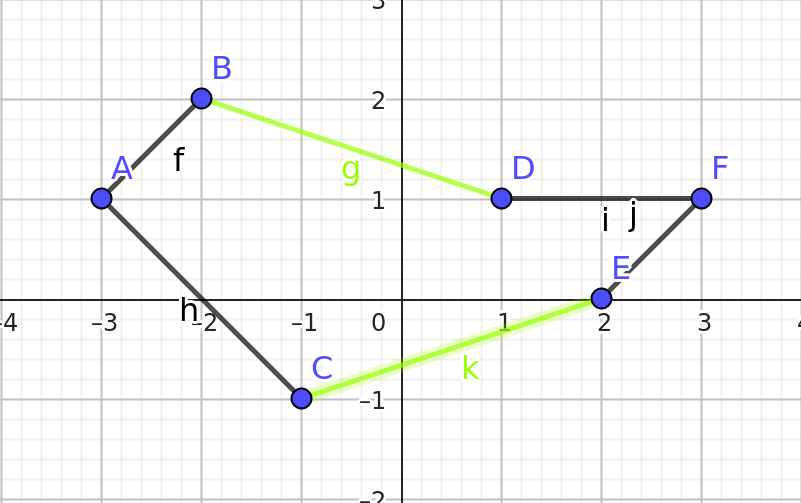
\includegraphics[width=\textwidth]{P3/Prosa/ej_unir1.png}
        \caption{\centering Opción 1}
        \label{fig:p3_ejemplo}
    \end{subfigure}
    \hfill
    \begin{subfigure}[b]{0.3\textwidth}
        \centering
        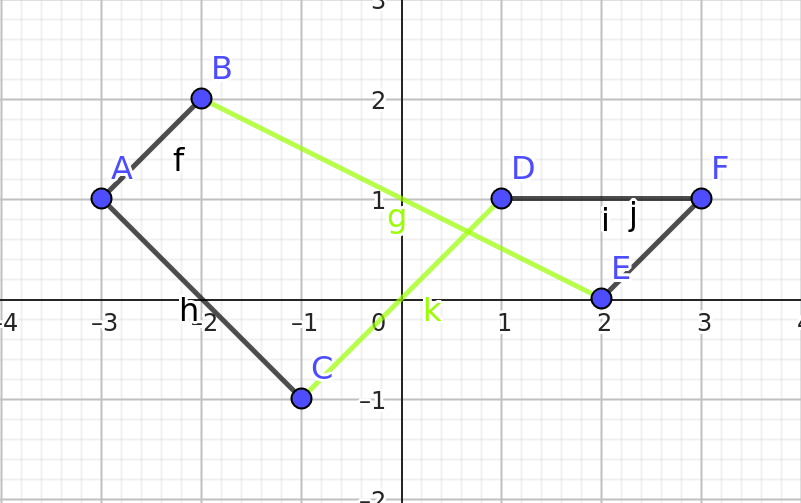
\includegraphics[width=\textwidth]{P3/Prosa/ej_unir2.png}
        \caption{\centering Opción 2}
        \label{fig:p3_ejemplo}
    \end{subfigure}
\end{figure}
\end{enumerate}
Veamos el algoritmo más claro con el siguiente ejemplo:
\begin{figure}[H]
    \centering
    \begin{subfigure}[b]{0.3\textwidth}
        \centering
        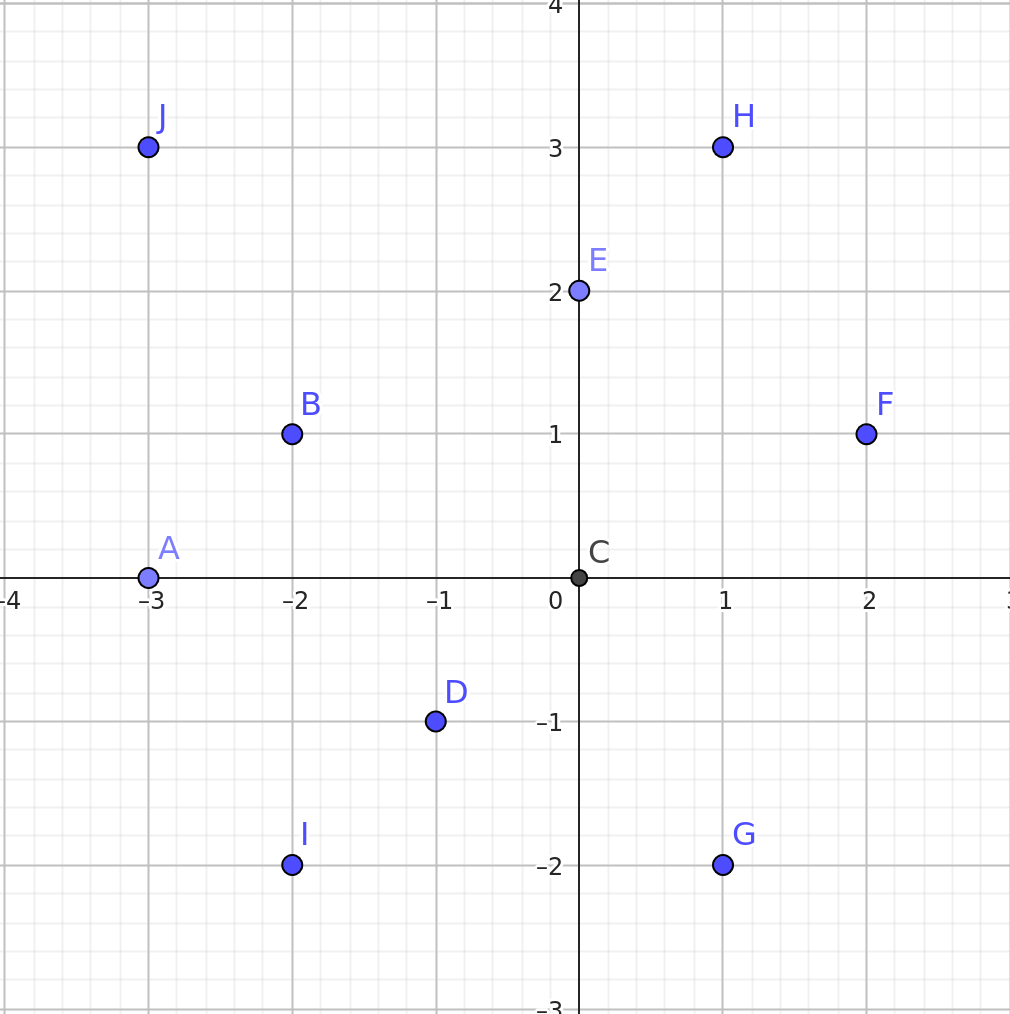
\includegraphics[width=\textwidth]{P3/Prosa/ejemplo.png}
        \caption{\centering Estado inicial}
        \label{fig:p3_ejemplo}
    \end{subfigure}
    \hfill
    \begin{subfigure}[b]{0.3\textwidth}
        \centering
        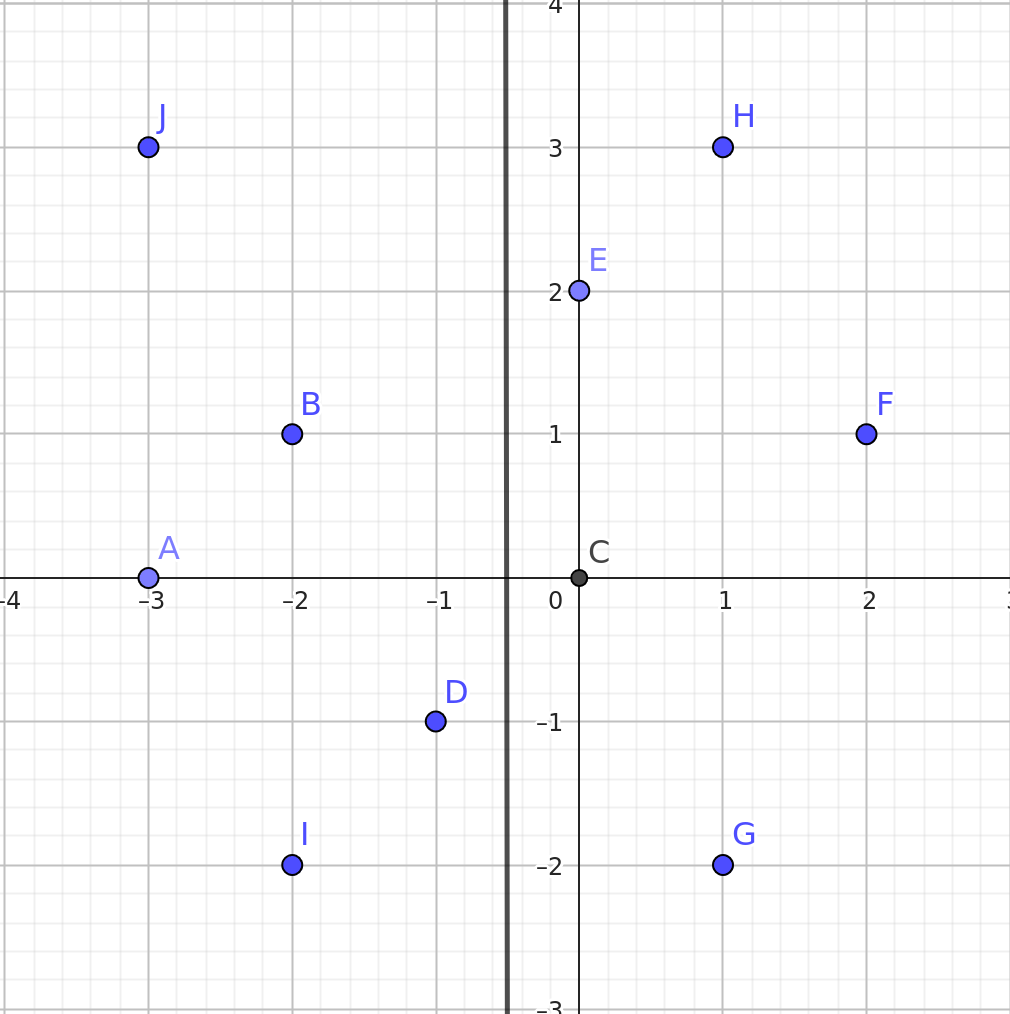
\includegraphics[width=\textwidth]{P3/Prosa/ejemplo_partir.png}
        \caption{\centering Partimos}
        \label{fig:p3_ejemplo}
    \end{subfigure}
    \hfill
    \begin{subfigure}[b]{0.3\textwidth}
        \centering
        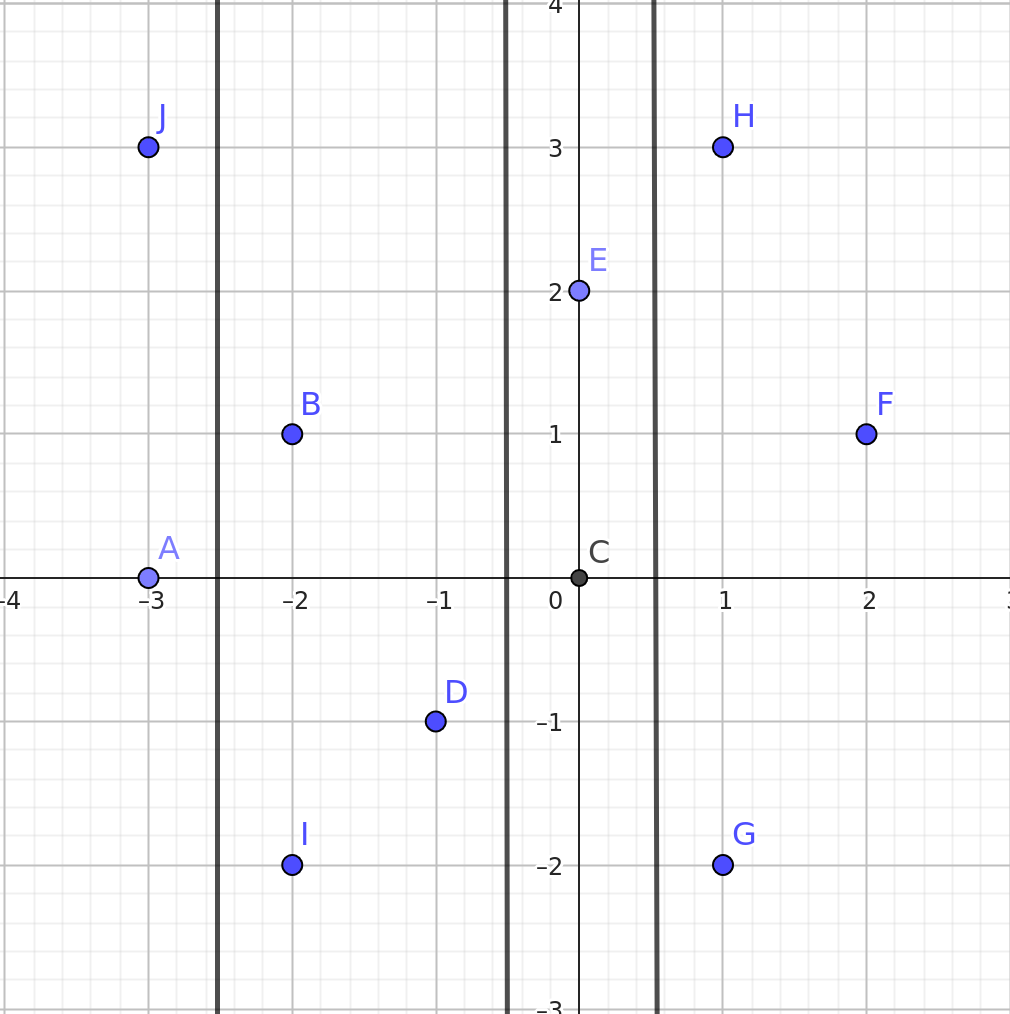
\includegraphics[width=\textwidth]{P3/Prosa/ejemplo_partir2.png}
        \caption{\centering Partimos de nuevo}
        \label{fig:p3_ejemplo}
    \end{subfigure}
    \newline
    \begin{subfigure}[b]{0.3\textwidth}
        \centering
        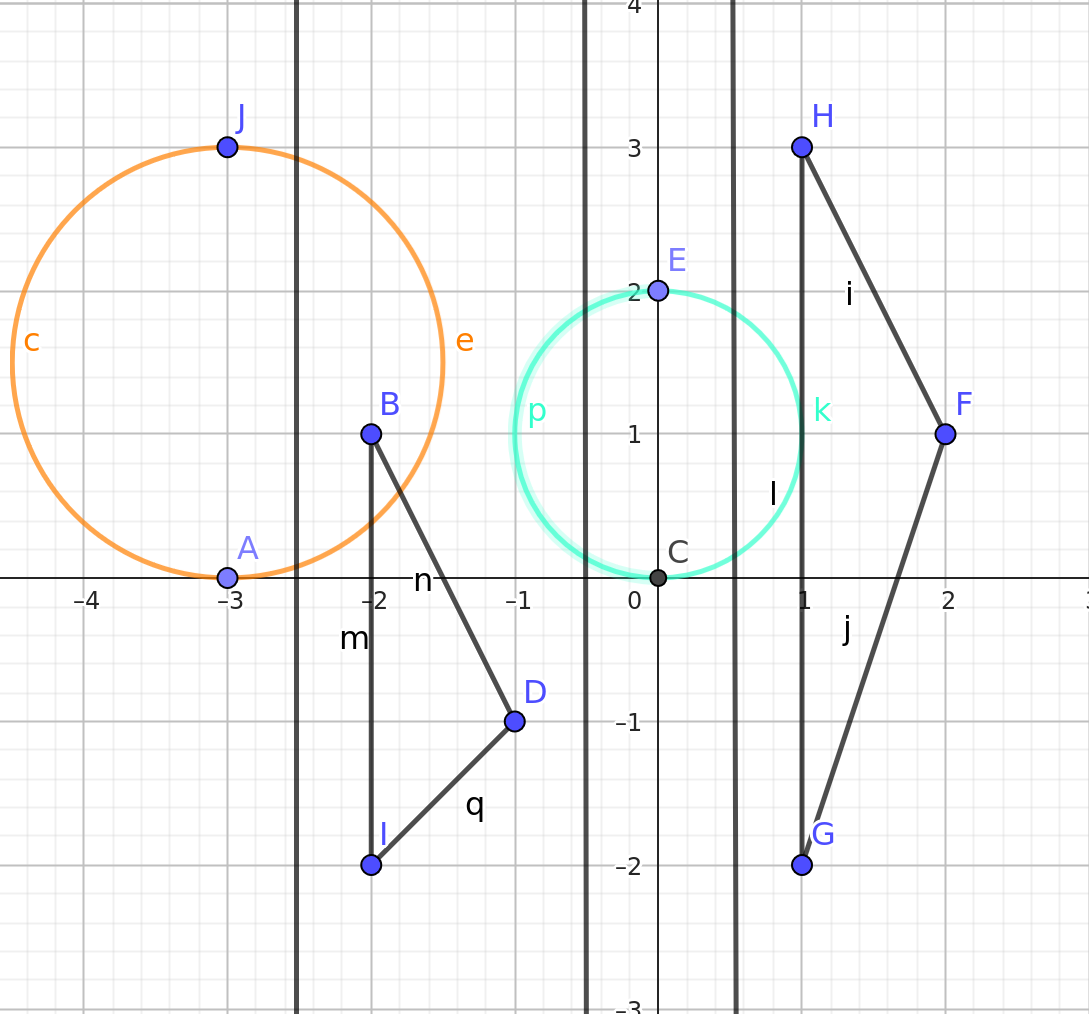
\includegraphics[width=\textwidth]{P3/Prosa/ejemplo_casos_base.png}
        \caption{\centering Casos base}
        \label{fig:p3_ejemplo}
    \end{subfigure}
    \hfill
    \begin{subfigure}[b]{0.3\textwidth}
        \centering
        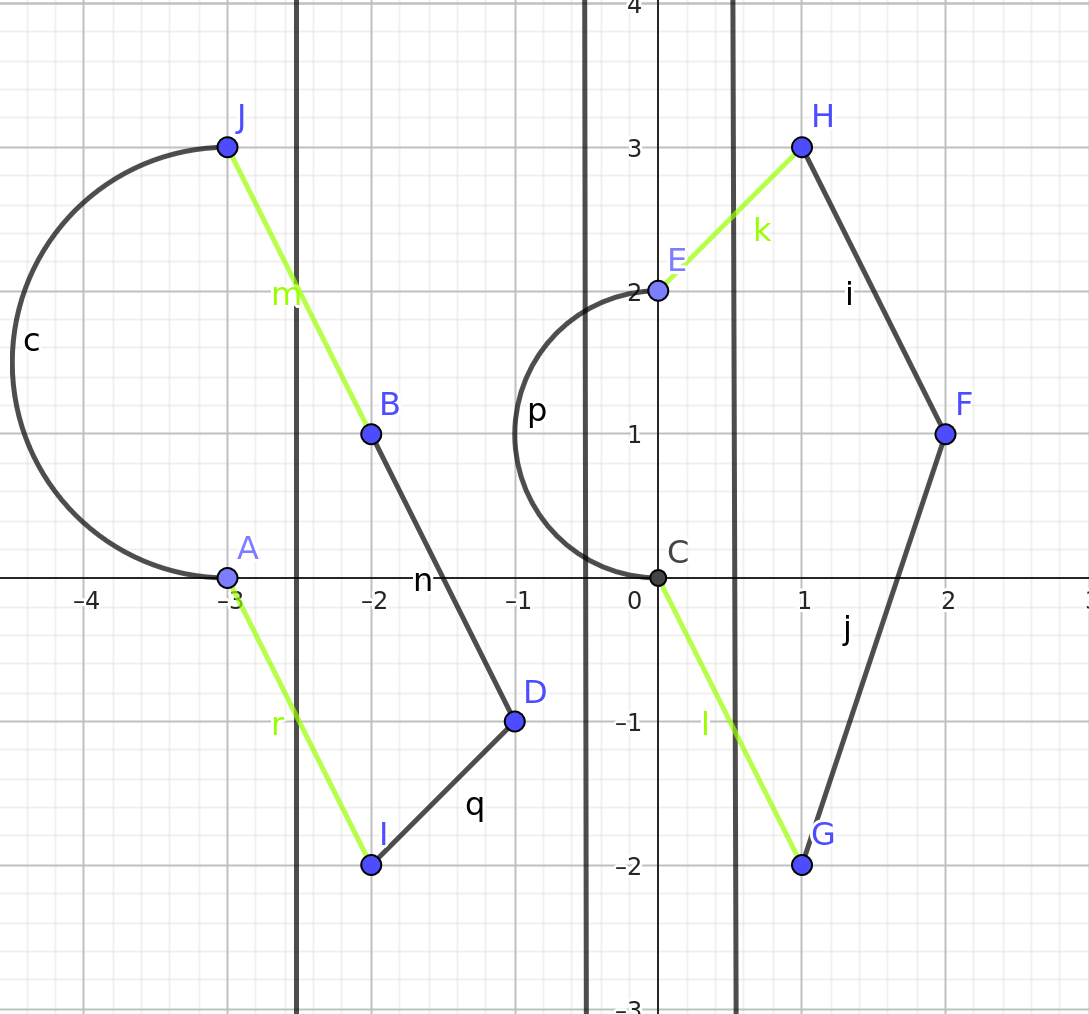
\includegraphics[width=\textwidth]{P3/Prosa/ejemplo_unir.png}
        \caption{\centering Unimos}
        \label{fig:p3_ejemplo}
    \end{subfigure}
    \hfill
    \begin{subfigure}[b]{0.3\textwidth}
        \centering
        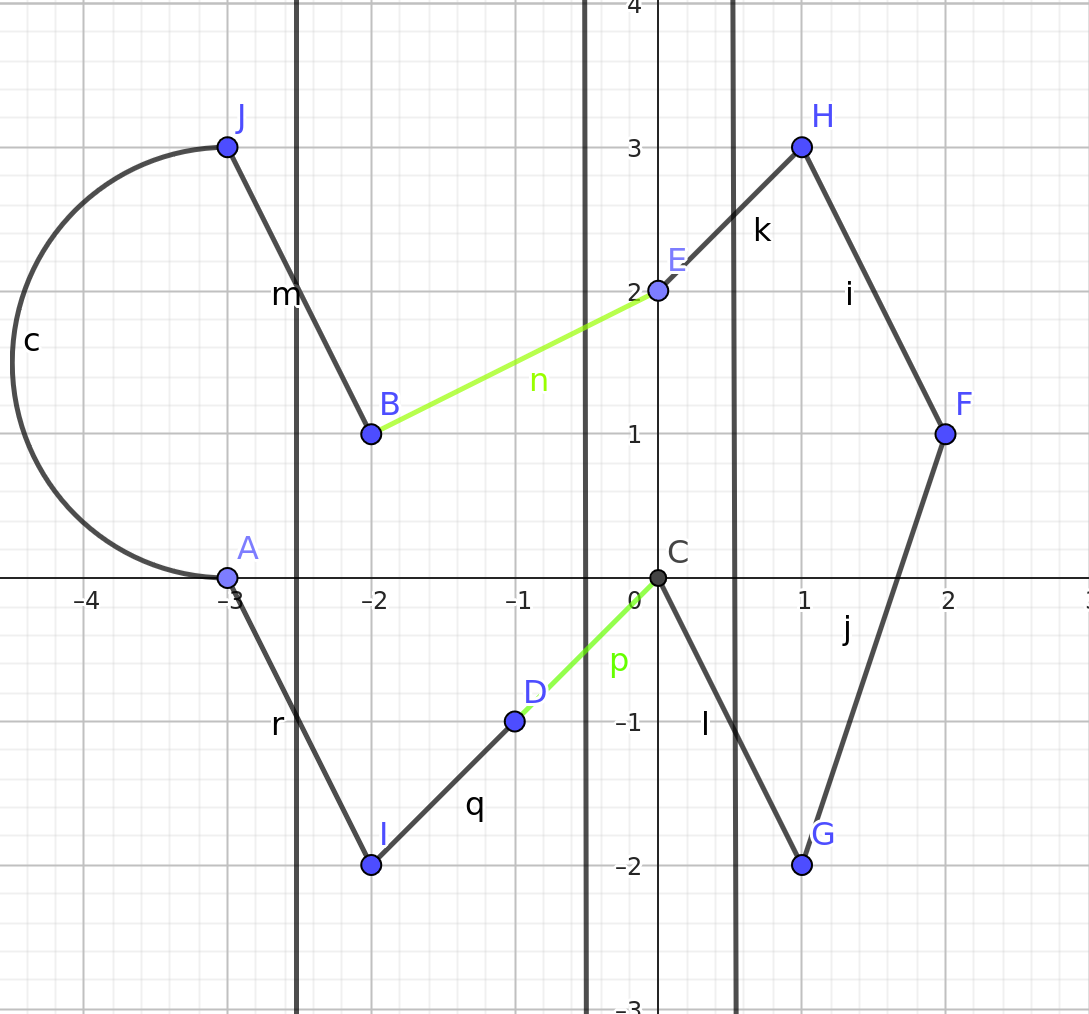
\includegraphics[width=\textwidth]{P3/Prosa/ejemplo_unir2.png}
        \caption{\centering Unimos de nuevo}
        \label{fig:p3_ejemplo}
    \end{subfigure}
\end{figure}

Como podemos observar, la solución dada por el algoritmo no es "mala" pero tampoco es la óptima. La solución óptima se puede ver el la figura \ref{fig:sol_optima}. Para ser exactos el coste del ciclo de nuestro algoritmo es 21.5853 mientras que el coste del ciclo óptimo devuelto por la solución específica es 20.8213. Por tanto el error cometido en este caso es: 
$$
error = \frac{(21.5853 - 20.8213) \cdot 100}{20.8213} = 3.6693194\%
$$

\begin{figure}
\centering
    \begin{subfigure}{0.3\textwidth}
        \centering
        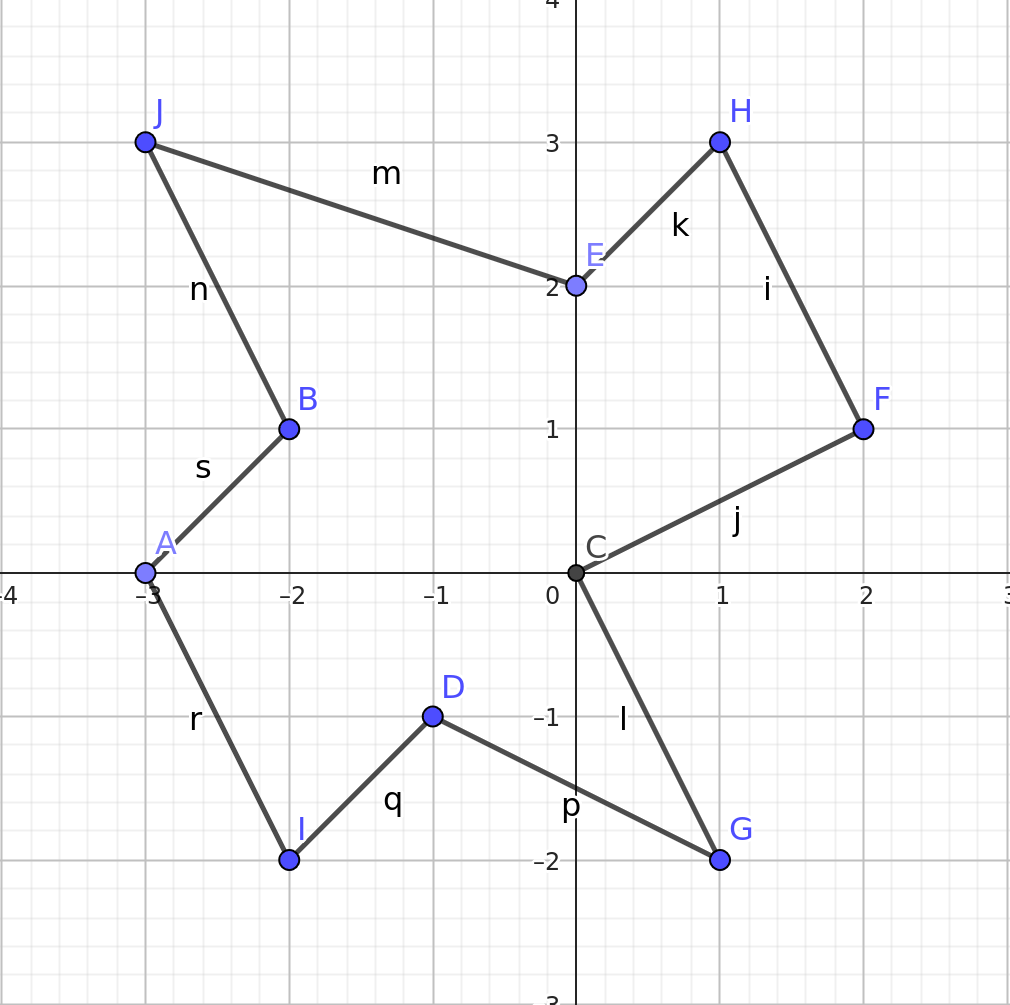
\includegraphics[width=\textwidth]{P3/Prosa/ejemplo_optimo.png}
        \caption{\centering Solución óptima}
        \label{fig:sol_optima}
    \end{subfigure}
    \begin{subfigure}{0.3\textwidth}
    \begin{verbatim}
        10
        (-3, 0)
        (-2, 1)
        (0, 0)
        (-1, -1)
        (0, 2)
        (2, 1)
        (1, -2)
        (1, 3)
        (-2, -2)
        (-3 ,3)
    \end{verbatim}
    \caption{\centering Input data}
    \end{subfigure}
\end{figure}

Hemos comparado el coste de la solución dada por el algoritmo divida y vencerás y el de la solución dada por el algoritmo específico que da la solución óptima para 1000 casos de pruebas de tamaño $n = 10$ (es decir, 10 ciudades) y la solución dada por el algoritmo divide y vencerás tiene de media un $26.15\%$ de error relativo (respecto al verdadero coste mínimo) con $\text{UMBRAL} = 4$. Con $\text{UMBRAL} = 2$ que se verá más adelante que es el umbral óptimo en tiempo de ejecución el error relativo medio es $27.38\%$.

\myparagraph{Implementación}
Para implementar este algoritmo, previamente a la llamada de la función que resuelve el algoritmo se ha ordenado el array de las ciudades en base a su coordenada $x$, de forma que las ciudades consecutivas son las más próximas respecto del eje X.
\lstinputlisting[language=C++, firstline=172,lastline=172]{Codigos/P3/dyv.cpp}
\begin{itemize}
    \item \textbf{Divide:}\\
    Nuestra forma de partir el problema ha sido dividir las ciudades por la mitad. Al estar las ciudades ordenadas por el eje X, tenemos que las ciudades que componen los dos grupos entre sí están relativamente próximas (lo están respecto del eje X por lo menos).
    \lstinputlisting[language=C++, firstline=68,lastline=72]{Codigos/P3/dyv.cpp}
    \item \textbf{Vencerás (fusión):}\\
    Tras las llamadas a la función tenemos el ciclo de coste mínimo de cada uno de los dos subgrupos. Como nuestro array de las ciudades está ordenado, podemos sabar en tiempo constante cuales son las 2 ciudades más próximas entre sí de ambos ciclos (1 de cada uno) ya que sus índices corresponden a los más cercanos al índice por el cual se partió el array. Por tanto, localizamos las ciudades dentro de sus respectivos ciclos.
    \lstinputlisting[language=C++, firstline=84,lastline=104]{Codigos/P3/dyv.cpp}
    Una vez localizadas, vemos cuales de sus ciudades adjadcentes está más centrada respecto a su coordenada $x$.
    \lstinputlisting[language=C++, firstline=106,lastline=122]{Codigos/P3/dyv.cpp}
    Tenemos entonces las 4 ciudades de ambos ciclos más cercanas entre sí conectadas si son del mismo ciclo. Si nuestras ciudades son $x$ e $y$ del primer ciclo y $z$ y $t$ del segundo, calculamos si es más barato uni $x$ con $z$ e $y$ con $t$ o $x$ con $t$ e $y$ con $z$.
    \lstinputlisting[language=C++, firstline=124,lastline=133]{Codigos/P3/dyv.cpp}
    Por último unimos ambos ciclos de la manera determinada en el paso anterior (sin olvidar romper la unión entre $x$ e $y$ además de $t$ y $z$, lo que implica restar estas distancias). La forma de unirlos es el primer ciclo desde $y$ hasta $x$ más el segundo ciclo desde $z$ hasta $t$ si $x$ se une con $t$ o al revés en caso contrario.
    \lstinputlisting[language=C++, firstline=135,lastline=154]{Codigos/P3/dyv.cpp}
\end{itemize}

%\lstinputlisting[language=C++, firstline=55, lastline=153]{Codigos/P3/dyv.cpp}

\subsubsection{Análisis de eficiencia} %

\myparagraph{Eficiencia teórica}

    Procedamos con el estudio de la eficiencia teórica. Definamos primero la función $T: \mathbb{N} \rightarrow \mathbb{R}$, donde dado el tamaño de entrada n, que es el número de ciudades a visitar, nos devuelve el tiempo empleado en ejecutar el programa que resuelve el problema con nuestro algoritmo. Viendo el código, es fácil ver 
    que toma la siguiente forma:

    \begin{equation} \label{eq:ef_dyv_p1}
    T(n) = \left\{ \begin{array}{lcc} n! & n \leq \text{UMBRAL}  \\ \\ 
    2T\left(\nicefrac{n}{2}\right) + n &  n > \text{UMBRAL}  \\ \end{array} \right. \hspace{10mm} \forall n \in \N
    \end{equation}

    Hay que tener en cuenta que estamos realizando un análisis con la notación O grande, por tanto, como el tiempo de ejecución del caso base está acotado por una constante, concluimos que es de la eficiencia O(1).
    En el caso general, vemos que realiza dos llamadas recursivas a la propia función con tamaño de entrada $\frac{n}{2}$ y, aparte de sentencias simples booleanas y condicionales de eficiencia O(1), realiza 8 bucles de tamaño $\frac{n}{2}$, 
    así utilizando la regla de la suma y del máximo concluimos que en el caso general nuestra función es de la forma $T(n) = 2T\left(\nicefrac{n}{2}\right) + n$. \\
    
    Para resolver esta recurrencia, realizamos un cambio de variable $n = 2^{m}$:

    \[
        T\left(2^{m}\right) = 2 \cdot T\left(2^{m-1}\right) + 2^{m} = 2 \cdot \left(2 \cdot T\left(2^{m-2}\right) + 2^{m-1}\right) + 2^{m} = 2^{2} \cdot T\left(2^{m-2}\right) + 2^{m} + 2^{m}
    \]

    Desarrollando k veces:
    
    \[
        T\left(2^{m}\right) = 2^{k} \cdot T\left(2^{m-k}\right) + k 2^{m}
    \]

    Teniendo en cuenta que $2^{m-k} \leq \text{UMBRAL} \iff m - \log_{2}{\text{UMBRAL}} \leq k $, tomamos $\bar{k} = [m - \log_{2}{\text{UMBRAL}}] + 1$, entonces $T\left(2^{m-\bar{k}}\right) =  (2^{m-\bar{k}})!$, desarrollamos: 
    
    \[
        T\left(2^{m}\right) = 2^{\bar{k}} \cdot T\left(2^{m-\bar{k}}\right) + \bar{k} 2^{m} 
                 = 2^{\bar{k}} \cdot (2^{m-\bar{k}})! + \bar{k} 2^{m} 
    \]

    Ahora, sustituyendo y deshaciendo el cambio de variable $m = log_{2}{n}$ y $\bar{k} = [m - \log_{2}{\text{UMBRAL}}] +~1$:
\begin{align*}
    T\left(2^{m}\right) &= 2^{\bar{k}} \cdot (2^{m-\bar{k}})! + \bar{k} 2^{m} \\
    &= 2^{ [m - \log_{2}{\text{UMBRAL}}] + 1} \cdot (2^{m-\bar{k}})! + ([m - \log_{2}{\text{UMBRAL}}] + 1) \cdot 2^{m} \\
    &= 2^{ [m - \log_{2}{\text{UMBRAL}}] + 1} \cdot (2^{m- [m - \log_{2}{\text{UMBRAL}}] - 1})! + ([m - \log_{2}{\text{UMBRAL}}] + 1) \cdot 2^{m} \\
    &= 2^{ [\log_{2}{n} - \log_{2}{\text{UMBRAL}}] + 1} \cdot (2^{\log_{2}{n} - [\log_{2}{n} - \log_{2}{\text{UMBRAL}}] - 1})! + ([\log_{2}{n} - \log_{2}{\text{UMBRAL}}] + 1) \cdot n  \\
    &= 2^{ [\log_{2}{n} - \log_{2}{\text{UMBRAL}}] + 1} \cdot (2^{[\log_{2}{\text{UMBRAL}}] - 1})! + ([\log_{2}{n} - \log_{2}{\text{UMBRAL}}] + 1) \cdot n \\
    &=T(n)
\end{align*}

    Como estamos trabajando con la notación O grande, nos interesa únicamente el comportamiento asintótico, y por tanto, ignorando las constantes:

    \[
         O(T(n)) = O(2^{\log_{2}{n}} + \log_{2}{n} \cdot n) = O\left(n + n\log_{2}{n}\right) = O\left(n\log{n}\right) 
    \]

    Por tanto, concluimos que nuestro algoritmo tiene una eficiencia teórica de $O(n\log{n})$.

\newpage
\myparagraph{Eficiencia empírica}

    Con el algoritmo implementado, ejecutamos el código con distintas instancias del problema (generados por el generador de casos),  y obtenemos la siguiente tabla:
    \begin{table}[H]
        \centering
        \begin{tabular}{|c|l|}
            \hline
            Nº ciudades & Tiempo (seg) \\
            \hline
            1000   & 0.000940859  \\
            11000  & 0.0117779    \\
            21000  & 0.0227117    \\
            31000  & 0.0317387    \\
            41000  & 0.0457       \\
            51000  & 0.0557699    \\
            61000  & 0.0632166    \\
            71000  & 0.0760993    \\
            81000  & 0.089748     \\
            91000  & 0.101802     \\
            101000 & 0.113085     \\
            111000 & 0.120791     \\
            121000 & 0.130018     \\
            131000 & 0.144707     \\
            141000 & 0.156846     \\
            151000 & 0.17327      \\
            161000 & 0.181568     \\
            171000 & 0.193043     \\
            181000 & 0.211589     \\
            191000 & 0.219642     \\
            201000 & 0.234674     \\
            211000 & 0.237546     \\
            221000 & 0.246918     \\ \hline
        \end{tabular}
        \caption{Tabla de tiempos de ejecución}
    \end{table}

    Como era de esperar, hemos definido como tamaño de entrada el número de ciudades. Ahora graficando los datos obtenemos las gráficas:

\begin{figure}[H]
    \begin{subfigure}{0.4\textwidth}
        \centering
        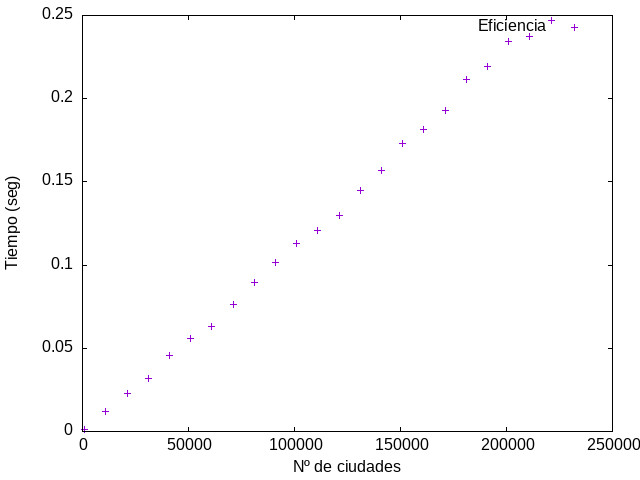
\includegraphics[scale = 0.40]{P3/pointsDyV.jpeg}
    \end{subfigure}\hfill
    \begin{subfigure}{0.4\textwidth}
        \centering
        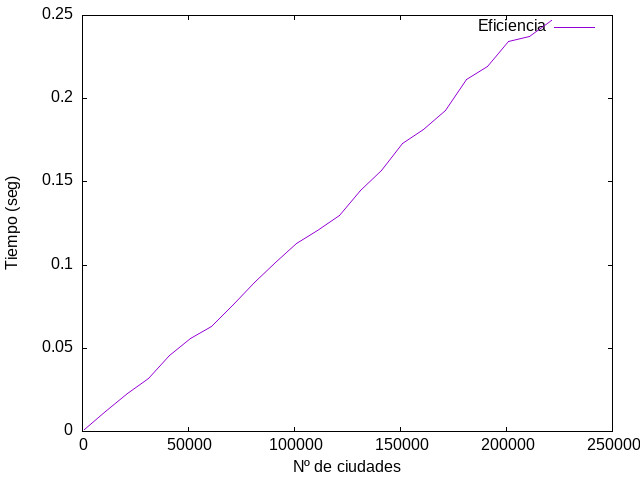
\includegraphics[scale = 0.40]{P3/linesDyV.jpeg}
    \end{subfigure}
\end{figure}

    Podemos observar que los datos siguen un crecimiento que parece o lineal o superlineal, y eso concuerda con el análisis teórico realizado, ya que el algoritmo es de eficiencia $O(n \log{n})$.

\myparagraph{Eficiencia híbrido}

    Veamos qué pasa si ajustamos una curva de regresión de la 
    forma $ f(x) = a_0 x \log{n} $ (función obtenida teóricamente) a los datos obtenidos 
    empíricamente:
    
    \begin{figure}[H]
        \centering
        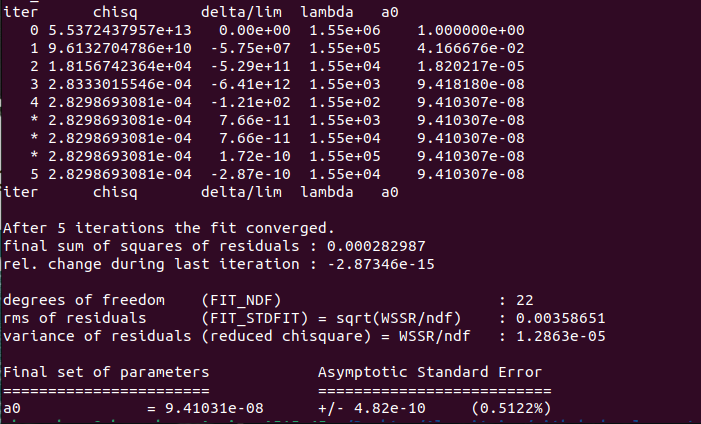
\includegraphics[width=0.5\linewidth]{P3/P3_regresionDyV.png}
    \end{figure}
    
   Vemos que con este ajuste, la varianza residual es practicamente nula, es decir, la curva se ajusta casi a la perfección a nuestros datos -- verificando nuestras conclusiones teóricas de que el algoritmo es de orden $O(n \log{n})$. 

   Graficando la función junto con nuestros datos obtenemos:

   \begin{figure}[H]
       \centering
       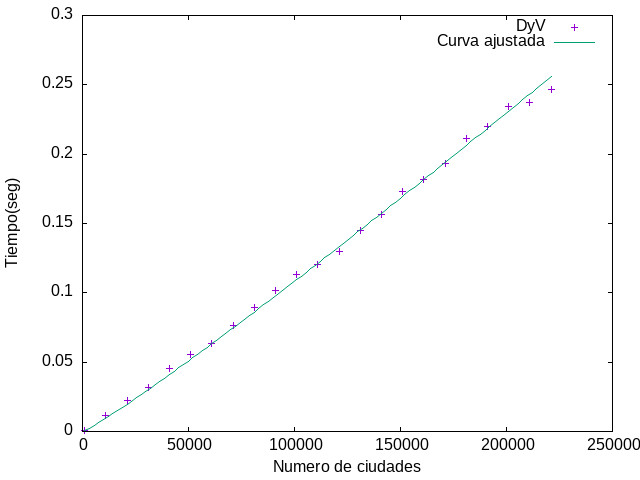
\includegraphics[scale=0.5]{P3/Curva_regresionDyV.jpeg}
       \caption{\centering $f(x) = 9.41\cdot10^{-8} x \log{x}$}
   \end{figure}

    \textbf{Conclusión:} En definitiva, nuestro algoritmo tiene la eficiencia calculada por el análisis teórico, y la curva de regesión se ajusta 
    a nuestros datos empíricos.
   
\subsubsection{Cálculo de umbrales} %
El problema del cálculo del umbral es de fundamental importancia
si pretendemos algoritmos rápidos usando la técnica \textit{Divide y vencerás}. Proponemos, como en los otro probleas, diferentes aproximaciones a la cuestión:
\myparagraph{Umbral teórico}    
Para el cálculo del umbral teórico procedemos como hemos visto en teoría: usando el tiempo de ejecución teórico del algoritmo
con la solución específica (fuerza bruta, en este caso) y 
la expresión recurrente del tiempo de ejecución para el método
recursivo con Divide y Vencerás (suponemos una única ejecución recursiva). 

Por tanto, tenemos que hallar $n_0$ tal que los siguientes
valores coincidan, y será el valor que pondremos
para el umbral teórico.
\begin{equation}
    T(n) = \left\{
	\begin{array}{lcc}
	    n! & \text{si } n \le \text{\text{UMBRAL}} \\
	    \\
	    2T\left(\nicefrac{n}{2}\right) + n & \text{si} n \ge \text{\text{UMBRAL}} \\
	\end{array}
	\right.
\end{equation} 
Es decir:
\
\[
    n_0\,! = 2\cdot\left( \frac{n_0}{2} \right) ! + n_0
\] 
Esta ecuación no es bajo ningún concepto fácil de resolver, y de hecho no tiene solución en los naturales. Sin embargo, numericamente obtenemos que, utilizando la extensión real con la función $\Gamma$ hay una solución alrededor de $2.93527687137463\ldots$ Así,
usaremos 3 como umbral teórico.

\myparagraph{Umbrales de tanteo}
Procedemos ahora a, habiendo obtenido un umbral teórico,
probar los tiempos de ejecución para diferentes umbrales cercanos
a éste. En particular, probamos con $\quad n_0 = 4 \quad n_0 = 5\quad n_0=2$ (que es el ya calculado) aparte de, claramente $n_0 = 3$. 
teórico.
\newline
Siguiendo exactamente el mismo procedimiento fue usado para el cálculo de la eficiencia empírica de los algoritmos, obtenemos la siguiente gráfica totalmente explicativa donde se comparan las ejecuciones con diferentes tamaños variando el umbral:

\begin{figure}[H]
    \centering
    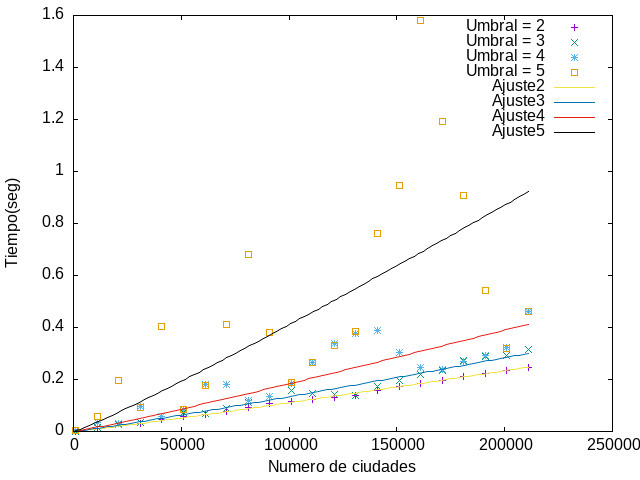
\includegraphics[scale=0.7]{P3/Umbral/dani_comparacion_umbrales.jpeg}
\end{figure}

Observamos de manera clara la diferencia de calidad entre los umbrales, siendo 2 y 3 de buena calidad y 4 y 5 (especialmente este último) de muy mala calidad, presentando unos resultados casi caóticos.
\newpage


\myparagraph{Umbral óptimo}

    Dado la expresión de la eficiencia híbrida del algorítmo específico, $5.110\cdot10^{-10} \cdot fact(n)$, lo igualamos con la expresión recurrente: 

    \[
        2\cdot T(\nicefrac{n}{2}) + n = 5.110\cdot10^{-10} \cdot fact(n)
    \]

    Aplicamos $T(\nicefrac{n}{2}) = 5.110\cdot10^{-10} \cdot fact\left(\nicefrac{n}{2}\right)$ :
    
    \begin{align*}
        &2\cdot 5.110\cdot10^{-10} \cdot fact\left(\nicefrac{n}{2}\right) + n = 5.110\cdot10^{-10} \cdot fact(n) \\
    \end{align*}

    Vamos a resolver esta ecuación emprícamente:


    \begin{figure}[H]
        \begin{subfigure}{0.4\textwidth}
            \centering
            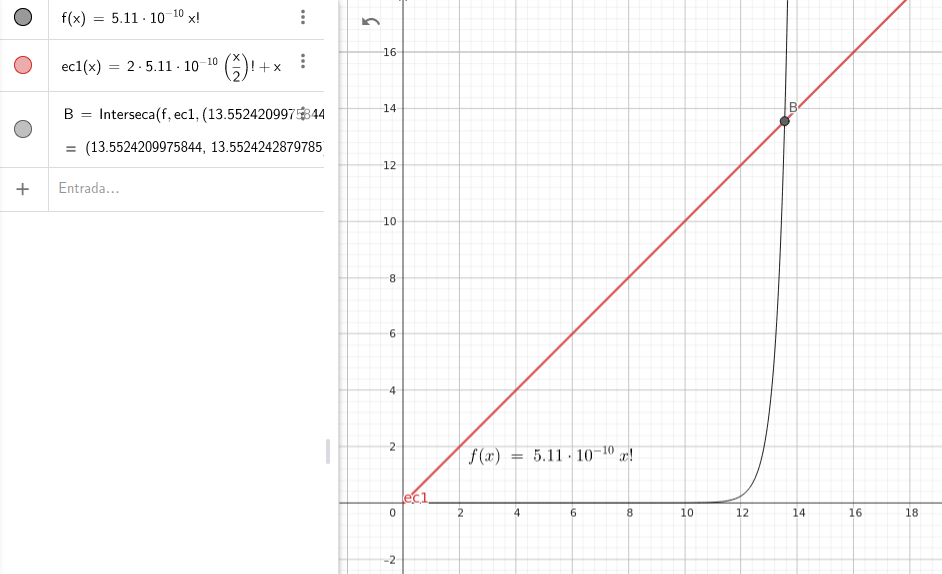
\includegraphics[width=0.9\linewidth]{P3/Geogebra/geogebra_analiatica4.png}
        \end{subfigure} \hfill
        \begin{subfigure}{0.4\textwidth}
            \centering
            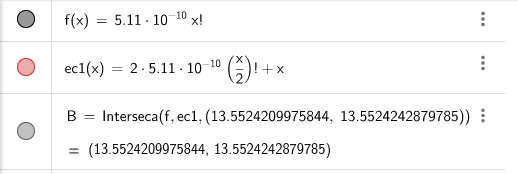
\includegraphics[width=0.9\linewidth]{P3/Geogebra/Analitico_Geogebra.png}
        \end{subfigure}
    \end{figure}
    
    Luego el umbral óptimo es \text{UMBRAL} = 13. \\

    A vista del comportamiento del algoritmo con los umbrales del tanteo y empírico, podemos deducir que con este umbral la eficiencia no va a ser la óptima. En el tanteo obtuvimos que el tiempo de ejecución empeoraba considerablemente cuando aumentabamos el umbral, que se aprecia con \text{UMBRAL} = 2,3,4,5. Además, cuanto mayor era \text{UMBRAL} veiamos que entre los tiempos de ejecución se producen más fluctuaciones, así, vamos a descartar el caso de \text{UMBRAL} = 13. 
    
\myparagraph{Umbral empírico}
    Vamos a comparar las gráficas obtenidas en los estudios de eficiencia híbrida del algoritmo de DyV y el esfecífico. 

    Si comparamos las gráficas obtenemos: 

    \begin{figure}[H]
        \begin{subfigure}{0.4\textwidth}
            \centering
            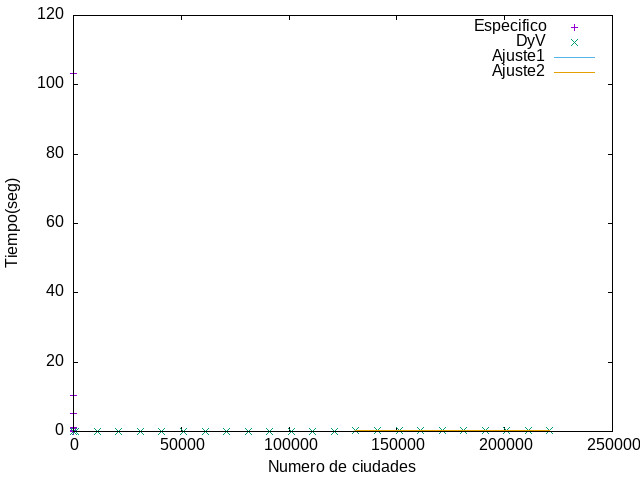
\includegraphics[scale = 0.40]{P3/Umbral/Salida_comparativa.jpeg}
        \end{subfigure} \hfill
        \begin{subfigure}{0.4\textwidth}
            \centering
            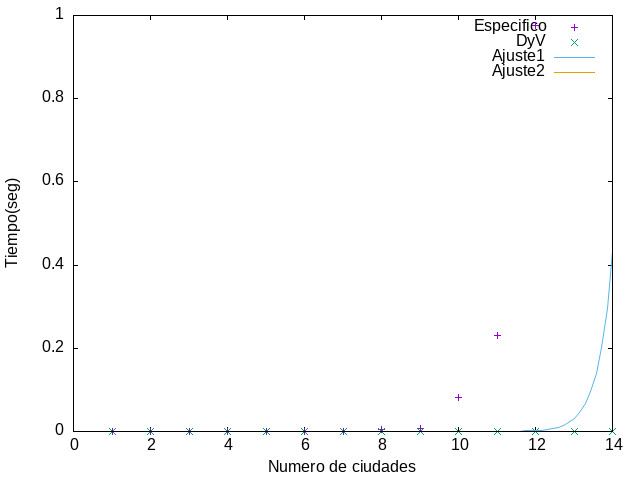
\includegraphics[scale = 0.40]{P3/Umbral/Salida_comparativa1.jpeg}
        \end{subfigure}
    \end{figure}

    Donde:
    \begin{itemize}
        \item Específico: son los datos obtenidos por la ejecución del algoritmo específico.
        \item DyV: son los datos obtenidos por la ejecución del algoritmo DyV.
        \item Ajuste1: es la curva de regresión obtenida para el algoritmo específico $Ajuste1(x) = 5.11\cdot 10^{-10} x!$.
        \item Ajuste2: es la curva de regresión obtenida para el algoritmo DyV $Ajuste2(x)= 9.14 \cdot 10^{-8} x \log(x)$. 
    \end{itemize}
    
    En la primera gráfica no es posible ver las curvas de regresión porque el Ajuste1 crece demasiado rápido y el Ajuste2 apenas crece.
    En la segunda gráfica es posible ver la curva que ajusta el algoritmo específico porque hemos cambiado la escala, pero aún así, la segunda curva crece demasiado, haciendo casi imposible visualizarla. \\
    Nota: El hecho de que podemos ver algunos datos de DyV es debido a que la curva de regresión se ajusta a todos los datos, y muy cerca de los entornos de algunos puntos (especialmente los primeros; donde hay bastante fluctuación de los tiempos de ejcución) la curva no se ajusta a la perfección. 
    
    \begin{figure}[H]
        \centering
        \includegraphics[scale=0.5]{P3/Geogebra/uwu_geobebra.png}
    \end{figure}

    Como ambas curvas intersectan en $x = 0.10$ que haciendo la parte entera de esta obtenemos que $n = 0$.
    
    Luego el umbral empírico es $n = 0$. 

\myparagraph{Grafica comparativa umbrales}

    Como para el caso de \text{UMBRAL} = 13 los resultados son poco satisfactorios, vamos a comparar única y exclusivamente los tiempos 
    de ejecución para \text{UMBRAL} = 1,2,3,4. No se compara \text{UMBRAL} = 5 porque se producen grandes fluctuaciones y la eficiencia es peor; y para \text{UMBRAL} = 0 (\text{UMBRAL} EMPÍRICO), pasamos a estudiar \text{UMBRAL} = 1, porque 1 es el mínimo valor de umbral posible. Y obtenemos la siguiente gráfica: 

    \begin{figure}[H]
        \centering
        \includegraphics[scale=0.75]{P3/Umbral/Imagen_UMBRAL_comparativa.jpeg}
    \end{figure}

    Observamos que resulta que el mejor umbral es \text{UMBRAL} = 2. Notemos que el error relativo con respecto a los umbrales empírico y teórico son del 50\%, un error bastante considerable, pero también tenemos que considerar que los valores de los umbrales obtenidos a comparar son muy pequeños, por tanto, las diferencias/errores relativas/os son muy sensibles a los cambios. 
    
    Ahora, también es lógico que los umbrales obtenidos tomen valores 
    pequeños, puesto que el algoritmo de DyV es $O(n\log(n))$ mientras 
    que el específico es $O(n!)$, es decir, la diferencia de eficiencia es considerable. \\
    Pero claro, tampoco hay que perder de vista que ganamos eficiencia a costa de aumentar el error de los resultados obtenidos(los caminos escogidos por el algoritmo específico son exactos mientras que los de DyV tienen unos porcentajes de error bastante considerables). Así, que el \text{UMBRAL} sea 2, no implica que la mejor calidad de los resultados se obtenga con dicho valor. 
    
\newpage

\section{Conclusiones}
A lo largo de esta investigación, hemos experimentado y validado la aplicabilidad y profundidad del paradigma \textbf{divide y vencerás} en la solución de problemas computacionales complejos, tal como se aborda en los contenidos teóricos de nuestra formación.

La práctica ha permitido no solo aplicar de manera concreta los principios teóricos sino también apreciar las significativas diferencias en términos de eficiencia que esta estrategia algorítmica aporta. Durante el proceso, nos hemos encontrado con comportamientos inesperados que resaltan la importancia de considerar las características específicas de los datos de entrada y las peculiaridades de la implementación en los resultados de los algoritmos. Así como verificar que la estrategia \textit{divide y vencerás} no es útil para cualquier caso ni tipo de algoritmo, sino para aquellos que son aptos para implementarse mediante esta técnica.

De manera particular, hemos observado la manifestación de conceptos teóricos clave en el desarrollo de nuestros algoritmos, tales como:
\begin{itemize}
    \item La relevancia de seleccionar implementaciones de algoritmos que consideren las implicaciones teóricas de su diseño, evitando ineficiencias como las generadas por llamadas recursivas excesivas.
    \item La constatación de que las variaciones en el tiempo de ejecución al cambiar de plataforma (ya sea por hardware o software) afectan fundamentalmente en una constante de proporcionalidad, manteniendo la relación de eficiencia entre diferentes algoritmos.
\end{itemize}

Esta práctica ha sido una valiosa oportunidad para trasladar la teoría al ámbito práctico, enfrentando desafíos reales y desarrollando una comprensión más rica de los principios algorítmicos. Consideramos que este ejercicio ha sido un éxito, enriqueciendo nuestra preparación para abordar futuras problemáticas en nuestro recorrido académico y profesional, dotándonos de herramientas y perspectivas cruciales para reconocer casos en los que la estrategia \textbf{Divide y Vencerás} sea viable, y saber cómo llevarlos al ámbito real y práctico en base a los conocimientos teóricos.

\end{document}
